\chapter{Designing the \ac{psa} and Antenna}
\label{chapter:design}

\par In this chapter, the choice of components used is explained. It is also detailed how the circuit was designed as well as the antenna that was used.

\section{Architecture}
\par One of the main objectives of this project was to develop a system that could be assembled as a set of blocks. This would help ensure high repeatability of the design. In this way, several replicas could be constructed with little difference between them.

\par The initial architecture for the design could be best described in Figure \ref{fig:ch_3_BlockDiagram.png}. In this diagram some characteristics of each block are already represented, as well as the component that was chosen and used for the prototype.

\begin{figure}[H]
    \vspace*{0cm}
    \centering
    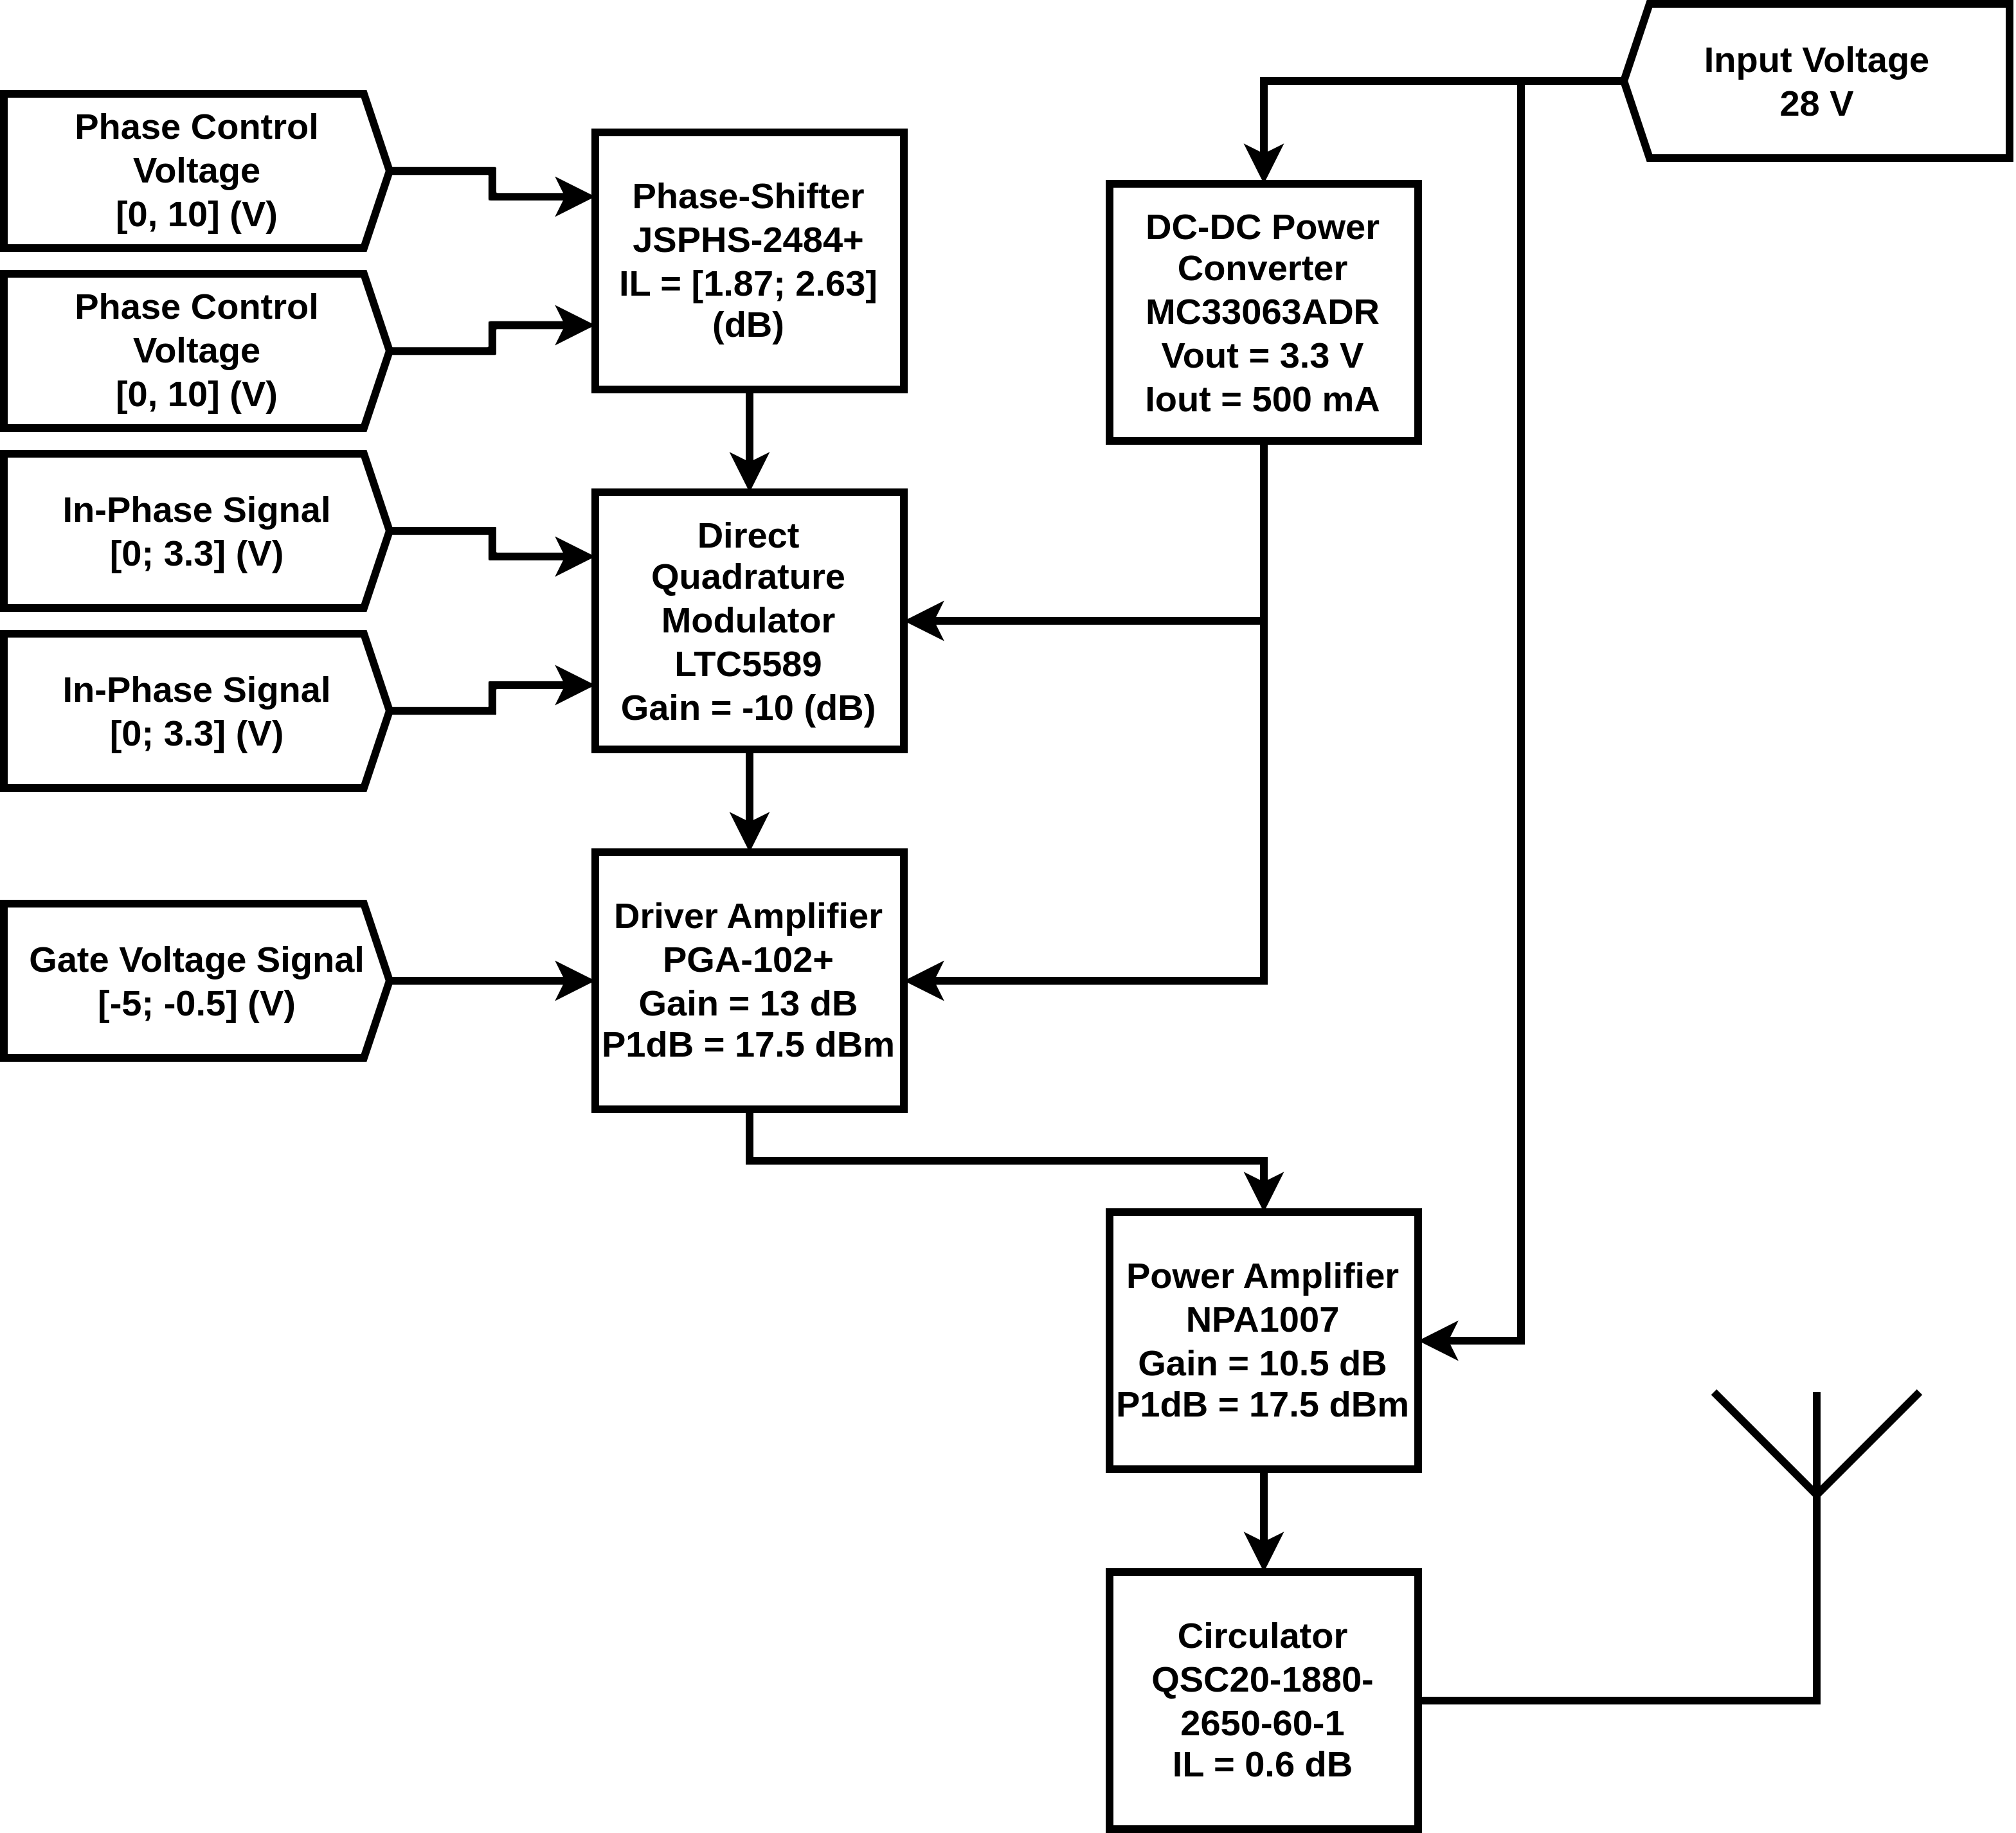
\includegraphics[width=0.9\linewidth]{figs/ch_3_BlockDiagram.png}
    \caption{Simplified Block Diagram of the system}
    \label{fig:ch_3_BlockDiagram.png}
\end{figure}

\par In order to work properly, the system would require a Phase Control Voltage signal for the Phase-Shifter. 

\par There would also be a 28V input to power the system that could later be used by the power converter to supply power to all components that would work at a different voltage than this. 

\par There was meant to also be present a signal that would be used to control the gate voltage for the power amplifier. This signal was meant to be supplied as a fixed $-5 \:\si{V}$ signal. The change in gate voltage would then be made by changing the position of a variable resistor.

\par Two signals would be provided, \acl{i} and \acl{q}. These signals did not impose any initial restrictions to the design of the project, so there was complete freedom in choosing their expected electrical characteristics. The choice of the modulator directly influenced this parameter. In the end, the LTC5589 modulator would use signals that had a common mode voltage from $1.4 \:\si{V}$ up to a maximum $2.0 \:\si{V}$, while the information carried by these two input signals, \ac{i} and \ac{q}, is presented in the differential mode (as there are two terminals for each input signal).

\par The carrier wave would be supplied directly to the phase-shifter. The initial restrictions for the frequency of operation were that it should be inside the range of $[2.4; 5.0] \:\si{GHz}$. This meant that choosing an appropriate component for this block would be easier, as this range is common. Another initial restriction that was discussed was that the phase-shifter would have to be capable of applying shifts in the range of $[0^{\circ}; 180^{\circ}]$ in order to be useful in the context of a \ac{psa} project.

\par The fact that no antenna would ever be perfect, as in with no return loss, means that there had to be a solution to prevent any reflection on the antenna returning to the power amplifier. There was also a concern that interference caused by neighboring elements, due to magnetic coupling, could negatively impact the operation of the \ac{pa}. These interference signals would could cause the a change in the impedance that the \ac{pa} sees at its output which could reduce the efficiency of the \ac{pa} and change its output power. To overcome these challenges, a circulator, here working as an isolator,  was placed on the output of the circuit, before the \ac{rf} signal is transmitted to the antenna.

\par Finally, from the beginning it was defined that the antenna would have a variation of a spiral antenna. This was due to limitations on the size of the antenna, as \ac{psa} benefit greatly of having its antenna elements at a distance of half the wavelength they will be radiating. Furthermore, spiral antennas have a larger bandwidth than patch antennas, while also having a lower directivity that allows the spiral antenna to have better beamforming performance.

\section{Choosing Components}
\par As mentioned previously, the components were mainly chosen with certain constraints in mind. There was an effort to find options that could be bought individually for the prototype phase, as it made no sense to acquire several units of a component that could end up being dropped from the design choice. During this phase, it also made sense to look for components that had larger stocks to facilitate future purchases.

\par There was also interest in trying to find all the components available from the same vendor. This would make the whole purchase procedure easier for Instituto de Telecomunicações.

\par It was also considered for all components if they would need additional purchases or circuits in order to work and if these were commonly available in online retailers or easy to implement and design.

\par Another factor that was kept in mind at all times was the monetary cost. Certain components could have been chosen and would require little to no effort in order to apply them to the project. However, their price was viewed as detrimental in the early stages of the veto process.

\par During selection, often a component would be considered initially as a viable option, but later down the line had to be reviewed as a newer component that had been chosen would either be incompatible with the previous choice or would require unnecessary steps to have them work together.

\subsection{The Phase-Shifter}
\par For the phase-shifter there are two main concerns from the start. First, it should be able to work at the desired \ac{rf} for the system. In this case, it should be able to accommodate a signal around $2.4\:\si{GHz}$. Also, this component would have to be able to change the phase of the signal up to $180^{\circ}$. 

\par Another factor that this component would have to respect would be its ability to be controlled by a voltage. So we were after a voltage controlled phase-shifter.

\par A search of online retailers with these characteristics in mind brought up a variety of components. The one that was chosen was the JSPHS-2484+ from Mini-Circuits. It fulfilled all the initial requirements, and still left some margins.

\par The fact that this component is not digitally controlled means that it is able to very precisely and accurately change the angle of the beam being radiated, while digital phase-shifters have a stepped output.

\par The graph in Figure \ref{fig:ch3_JSPHS-2484+PHASE_SHIFT.png}, presented in the datasheet, details how the phase shifts with the variable voltage control signal for various frequencies.

\begin{figure}[H]
    \vspace*{0cm}
    \centering
    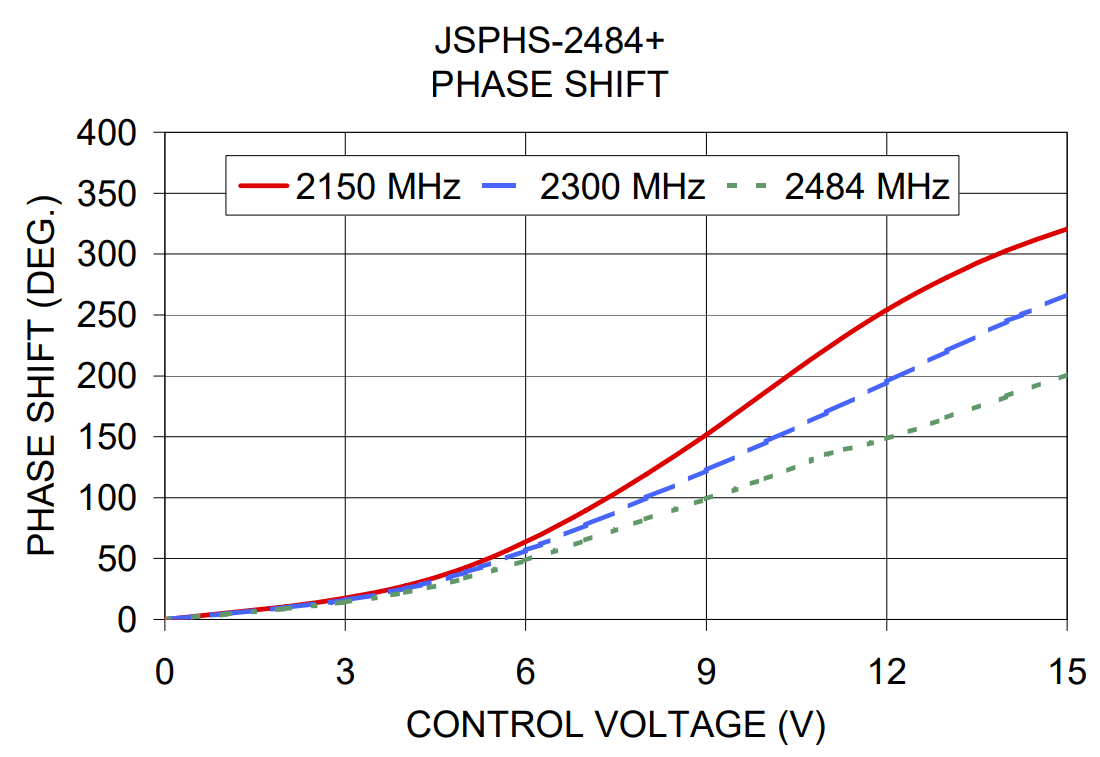
\includegraphics[width=0.6\linewidth]{figs/ch3_JSPHS-2484+PHASE_SHIFT.png}
    \caption{Phase shift (\textdegree) vs Control voltage (V) \cite{PhaseJSPHS-2484+}}
    \label{fig:ch3_JSPHS-2484+PHASE_SHIFT.png}
\end{figure}

\par In this project we are mostly interested in the two frequencies of $2300\:\si{MHz}$ and $2484\:\si{MHz}$ that are shown, up to a maximum of $180^{\circ}$. By analyzing this graphic we can conclude that it would satisfy the goals set for the phase-shifter.

\par Unfortunately, there are other characteristics that can also influence the behavior of the phase-shifter and how it can be integrated into the project. The major two factors  being its \ac{vswr} and \ac{il}. Figures \ref{fig:ch3_JSPHS-2484+VSWR.png} and \ref{fig:ch3_JSPHS-2484+INSERTION_LOSS.png} show two graphs present in the phase-shifter datasheet that detail how these factors change with the \ac{rf} used and the control voltage.

\begin{figure}[H]
    \vspace*{0cm}
    \centering
    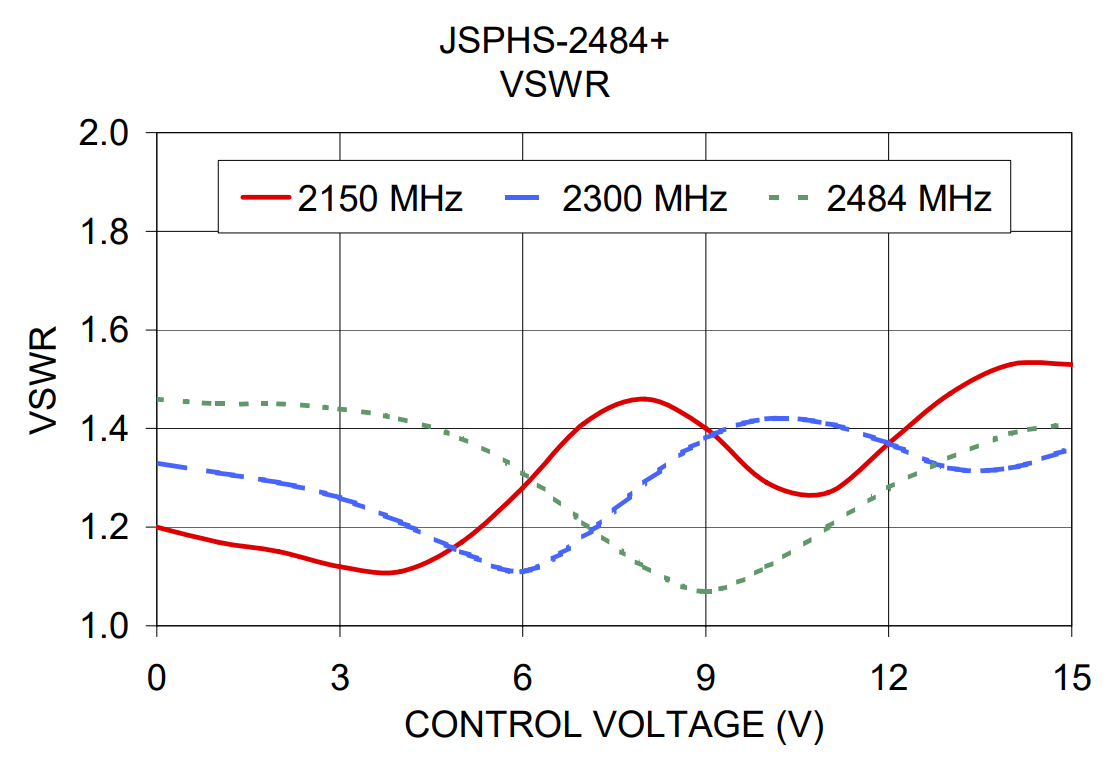
\includegraphics[width=0.6\linewidth]{figs/ch3_JSPHS-2484+VSWR.png}
    \caption{VSWR of JSPHS-2484 \cite{PhaseJSPHS-2484+}}
    \label{fig:ch3_JSPHS-2484+VSWR.png}
\end{figure}

\par We can assume that for the operation conditions that the phase-shifter will be subject in our project, its maximum value for \ac{vswr} would be, rounding up for simplicity, at around $1.5$ for a frequency of $2484 \:\si{MHz}$ when the control voltage is null.

\par Now, the maximum power that the JSPHS-2484 can handle at its \ac{rf} input is $ 20 \:\si{dBm}$.  At the specified \ac{vswr} the power loss in the phase-shift is around $6 \:\si{dBm}$, or $\:\si{0.004W}$. Although not desirable, this amount of power would not necessarily be harmful to the system.

\begin{figure}[H]
    \vspace*{0cm}
    \centering
    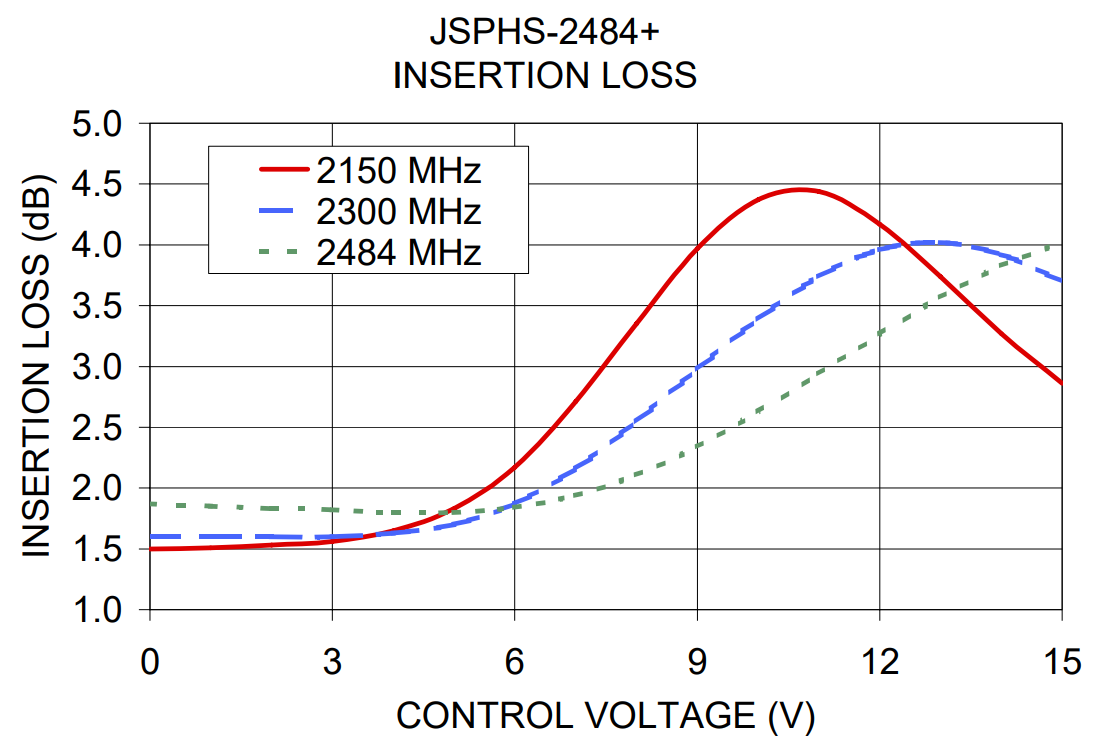
\includegraphics[width=0.6\linewidth]{figs/ch3_JSPHS-2484+INSERTION_LOSS.png}
    \caption{\ac{il} for JSPHS-2484 \cite{PhaseJSPHS-2484+}}
    \label{fig:ch3_JSPHS-2484+INSERTION_LOSS.png}
\end{figure}

\par The most significant of these factors is the \ac{il} as it increases significantly for the desired \ac{rf} reaching almost $3.4 \:\si{dB}$.

\subsection{Quadrature Modulator}
\par For the modulator, the frequency of operation was also a concern. It had to be able to support a carrier signal at a frequency of \ac{rf}.

\par But there was another characteristic that had been specified during the initial phase of the project. The \ac{i} and \ac{q} components that would be be fed to the modulator would operate at a maximum frequency of $20 \:\si{MHz}$. These two requirements alone would help narrow down the list of possible alternatives for this component choice.

\par Another important parameter that was considered was the total power consumed. Some of the devices that were in a convenient price range would have a total power consumption that would be considered somewhat high, at around $900 mW$. Due to the fact that the system would be encapsulated within a compact enclosure, this could be considered a problem. The unnecessary heat added to the heat already expected to be generated by a $10 W$ \ac{pa} could be a problem.

\par In the end, the LTC5589IUF from Analog Devices was chosen as what was thought to be the appropriate quadrature modulator to be used for the project.

\par Unfortunately, during the vetoing of this component, two I made two oversights. The first was to misunderstand the output power of this device. This lead to the belief that the LTC5589IUF would have a gain of $0 \:\si{dB}$, meaning that the signal at the output would have the same power as at the input. In reality, the gain of this device can be interpreted from the following graph taken from the datasheet of the component that is present in Figure \ref{fig:ch3_GainVCTRLquadmod.png}. The gain would actually be closer to $-10 \:\si{dB}$, as the parameter $V_{CTRL}$ was set at $3.3 \:\si{V}$ in the designed prototype.

\begin{figure}[H]
    \vspace*{0cm}
    \centering
    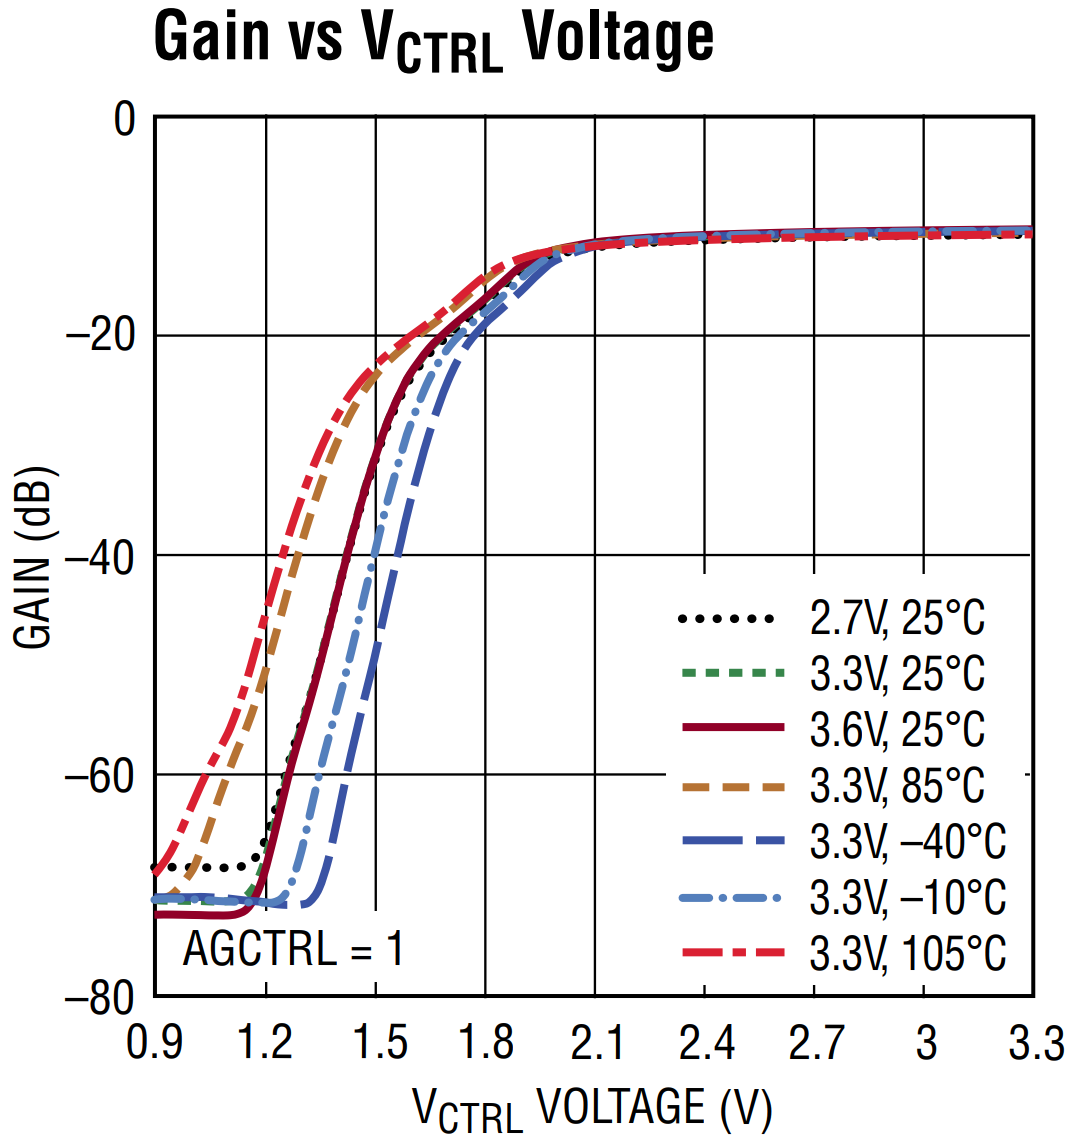
\includegraphics[width=0.6\linewidth]{figs/ch3_GainVCTRLquadmod.png}
    \caption{Relationship of analog gain with $V_{CTRL}$ \cite{LTC5589}}
    \label{fig:ch3_GainVCTRLquadmod.png}
\end{figure}

\par Another characteristic of the LTC5589IUF modulator, and, in fact, of other component used in the project, was its footprint and size. This component is in a QFN package with $4 \:\si{mm}$ sides, with 24 total leads and a thermal pad. Even with the help of Professor Telmo Cunha and the technical expertise of Paulo Gonçalves, it would turn out to be a rather complicated component to properly solder onto the \ac{pcb}. 

\par Another modulator that could have been used would have been the TRF3705IRGET from Texas Instruments. This component can work at the desired frequency, had a gain of approximately $2 \:\si{dB}$ at $2.6 \:\si{GHz}$ and could achieve a maximum output of $6.5 \:\si{dBm}$ at $2.4 \:\si{GHz}$. However, this would also be a QFN package component, which means that the soldering procedure would remain rather difficult. The only major mechanical difference between the TRF3705IRGET and the LTC5589IUF is that the pad underneath the component is thermal rather than connected to ground. This pad is needed because the component will consume more $276.5 \:\si{mA}$ over the LTC5589IUF, totaling $306 \:\si{mA}$.

\subsection{Power Supply} 
\par At this point, there were enough known variables about the project that the choice for a suitable component and subsequent circuitry could be made. The supplied voltage would be $28 \:\si{V}$ and the modulator would work at a supply voltage of $3.3 \:\si{V}$. As such, there was a need to find a component that could be used in a \ac{smps}. This \ac{smps} would be configured as a Buck converter.

\par These two constraints alone were enough to narrow down the number of possible components to be used for the project quite significantly.

\par After some considerations regarding the possibility of a driver amplifier for the \ac{pa}, the switching regulator MC33063ADR from Texas Instruments was chosen. The MC33063ADR could handle up to $1.5 \:\si{A}$ output current with an efficiency of around $83.7\%$. 

\par It could achieve this without the need for many external components. The simplified schematic of this component is presented in the datasheet shown in Figure \ref{fig:ch3_smpsInternal.png}.

\begin{figure}[H]
    \vspace*{0cm}
    \centering
    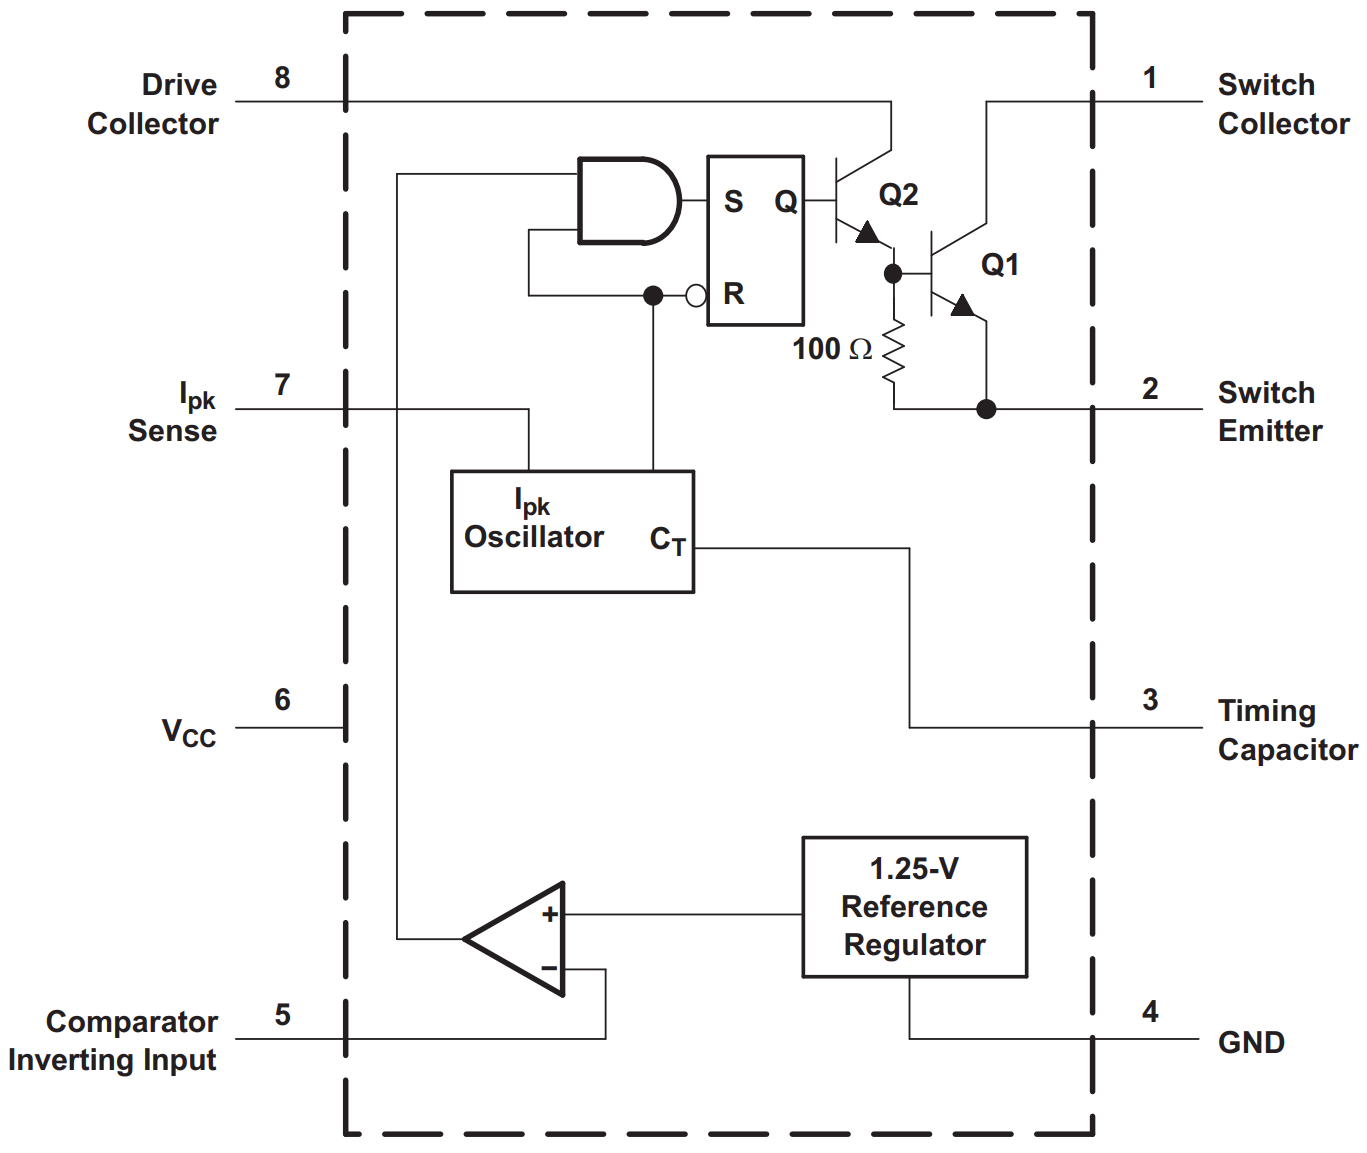
\includegraphics[width=0.6\linewidth]{figs/ch3_smpsInternal.png}
    \caption{Simplified schematic for the MC33063ADR switching regulator \cite{2004MC3x063ARegulators}}
    \label{fig:ch3_smpsInternal.png}
\end{figure}

\par As we can see, the MC33063ADR is a package that already has the internal circuitry needed for many of the requirements of a basic buck converter. There would be no need for external transistors, comparator, oscillator, or voltage references. However, it would require other components depending on the application.

\subsection{Driver Amplifier}
\par For this driver amplifier, some desirable characteristics were considered during selection. The first was the operating frequency range. It had to include the desired \ac{rf} of $2.4 \:\si{GHz}$. Secondly, all the components that had been chosen so far would require a supply voltage of $3.3 \:\si{V}$, so the driver amplifier would be limited to this voltage.

\par As a driver amplifier, this component would be expected to have a high enough gain, since \ac{pa} are often lacking in this parameter.

\par Another factor that influenced the decision process was how easy the amplifier would be to integrate with the rest of the circuit. Meaning, if there was any need for matching any ports, as the initially thought process behind the project would be to try and assemble the whole system with the most ease.

\par After searching through the major online retailers, it was decided on the PGA-102+ monolithic amplifier from Mini-Circuits. 

\par This amplifier can work with the supply voltage of $3.3 \:\si{V}$ and uses a maximum of $83 \:\si{mA}$ It advertises a gain of approximately $13 \:\si{dB}$ at $2.4 \:\si{GHz}$ with a P1dB of $17.5 \:\si{dBm}$ at this frequency. Unfortunately, it was noticed after the circuit was assembled that this low P1dB would limit the output power of the circuit to a maximum of approximately $28 \:\si{dBm}$, which was lower than expected.

\par This amplifier was already matched internally, which meant that its application would be easier. 

\par However, this amplifier would still require some external components for proper \ac{rf} applications. A bias-tee and some block or bypass capacitors would need to be present, according to the manufacturer, as can be seen in the recommended application circuit from the datasheet shown in Figure \ref{fig:ch3_pga102+application.png}. 

\begin{figure}[H]
    \vspace*{0cm}
    \centering
    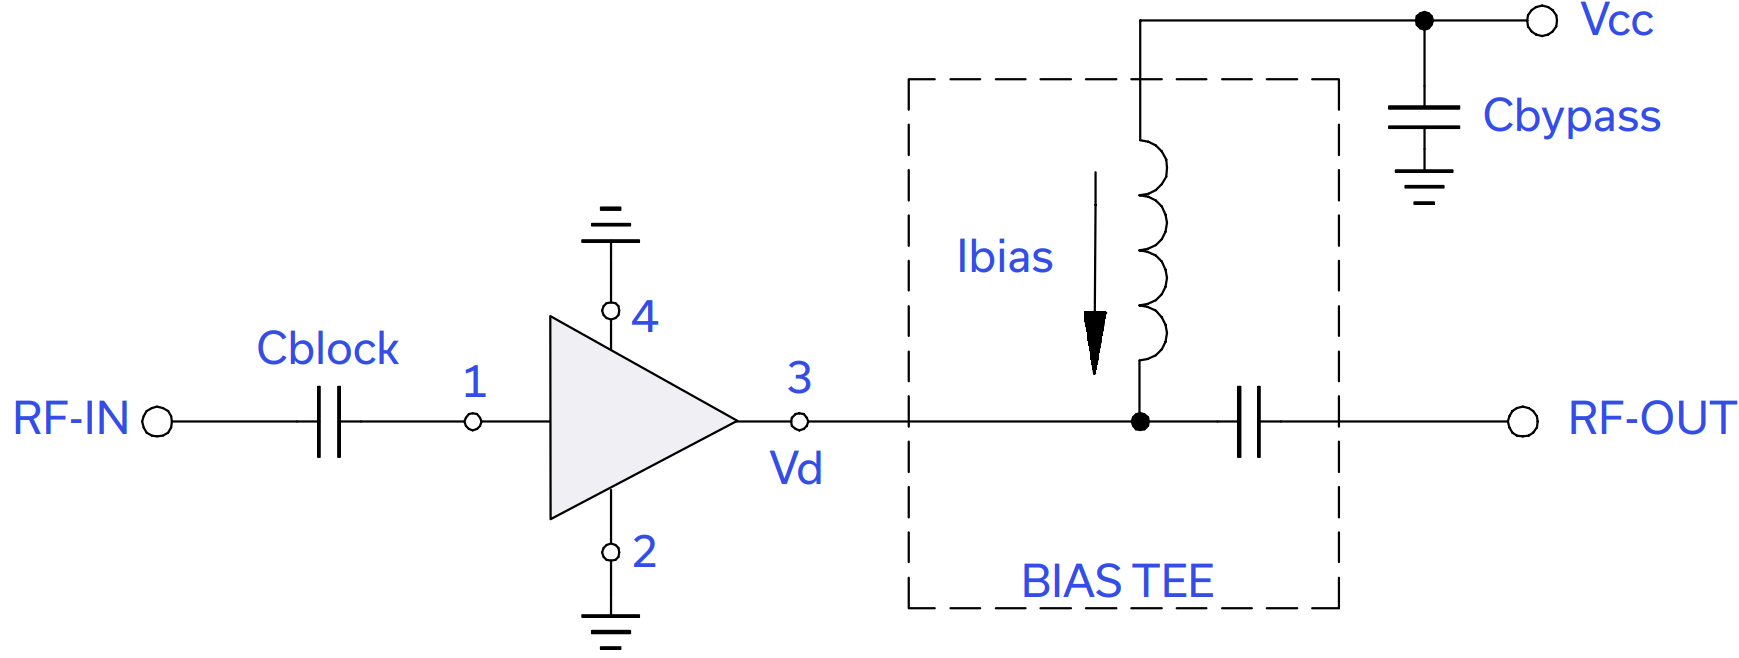
\includegraphics[width=0.7\linewidth]{figs/ch3_pga102+application.png}
    \caption{Recommended application circuit for a PGA-102+ \cite{MonolithicPGA-102+}}
    \label{fig:ch3_pga102+application.png}
\end{figure}

\par This, however, did not pose a concern that could overthrow the choice made for this component.

\subsection{\textbf{\ac{rf} Power Amplifier}}
\par This component is one of the more important ones in the project. It would need to provide most of the power to the signal that goes out to the antenna. Firstly, this amplifier would be required to be able to deliver the expected $40 \:\si{dBm}$ of peak power.

\par With this in mind and with all other constraints related to the operation of the project, in the end the NPA1007 \ac{pa} from MACOM was chosen. This device provides $10.5 \:\si{dB}$ of gain at an input power of $30 \:\si{dBm}$.

\par This amplifier also has its input already matched, which means that it is only required to match the output of the amplifier. The datasheet already details how this can be done. The datasheet also details the procedure for turning on and off the device. 

\par Unfortunatly, the drain efficiency of the amplifier for the desired output power is around $40\%$. This means that a lot of power will be turned into heat. For an operating output power of $40 \:\si{dBm}$ it would be expected to produce around $13 W$ of heat.

\subsection{Enclosure}
\par As mentioned previously, the idea would be for each element of the array to be as close to each other as possible in order for the antennas to be spaced about half a wavelength from each other. For an application at $2.4 \:\si{GHz}$, this means a distance of around $6.3 \:\si{cm}$ or $2.46 \:\si{in}$, rounded up to the millimeter. This measure would be critical, as it would determine the maximum width and height of the enclosure. There was no restriction for the total depth of the box, as long as it was reasonable. Ideally, this enclosure would be metal so that the circuits inside could be shielded. But after an unsuccessful search, this criteria was abandoned, and the search also started including other materials.

\par There was also the fact that this enclosure would have to undergo some modifications if we wanted to have some sort of front panel connections on one side of the box, and leave a whole to properly bias the power amplifier.

\par In the end, the Bud Industries CU-793-MB model was chosen as a suitable enclosure. This box has a width of $2.23 \:\si{in}$, or $5.66 \:\si{cm}$, on the top that then tapers to $2.125 \:\si{in}$, or $5.4 \:\si{cm}$, on the bottom, as can be seen in Figure \ref{fig:ch3_CU-793-MB.png}. This box has a depth of around $4 \:\si{in}$, or $10.16 \:\si{cm}$.

\begin{figure}[H]
    \vspace*{0cm}
    \centering
    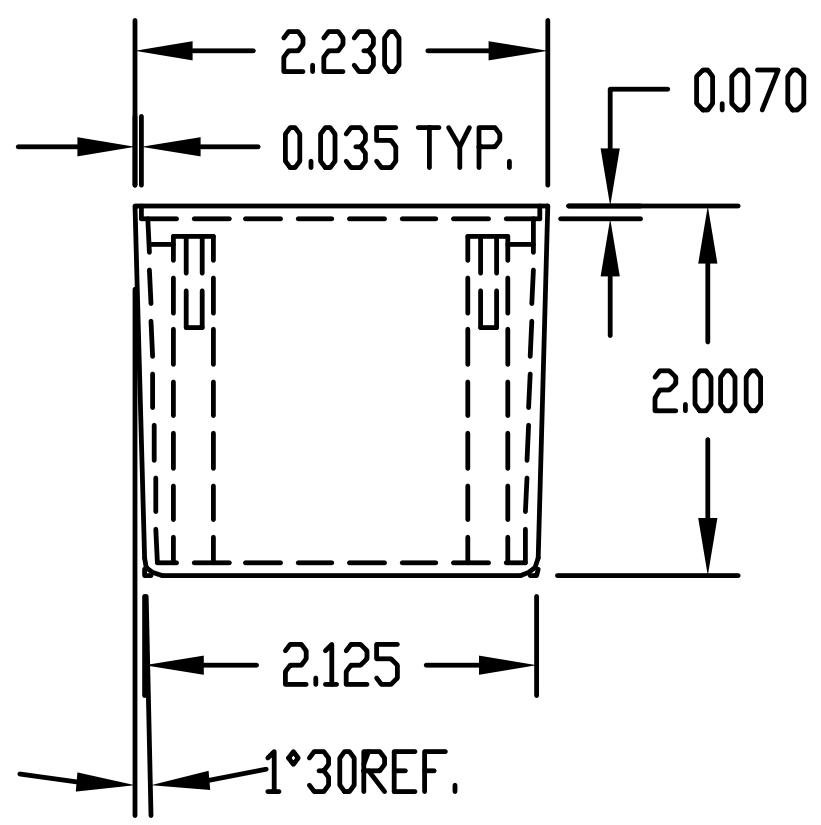
\includegraphics[width=0.4\linewidth]{figs/ch3_CU-793-MB.png}
    \caption{Dimensions of the external face of the enclosure \cite{UtiliboxCUR-793}}
    \label{fig:ch3_CU-793-MB.png}
\end{figure}

\par This choice will also set the limits for the future \ac{pcb} to be used for the project.

\subsection{Connectors and \ac{pcb} substrate}
\par For the substrate of the \ac{pcb}, we will use the same that is recommended by MACOM to the NPA1007 \acl{pa}. It is the Rogers RO4350B with a thickness of $0.508 \:\si{mm}$.

\par One of the requirements of this project would be to be able to have all the signals delivered to the array element via a front panel. To do this, we would have to bridge the gap from the \ac{pcb} to the outside. 

\par For the carrier wave signal, this could be done by simply adding an SMA connector to the edge of the \ac{pcb} and drilling a hole in the box, having it protrude in order to be accessible from the outside. The connector used is CON-SMA-EDGE from FR Solutions.

\par To deliver the \ac{iq} signals, as it would be impossible to mount many more connectors on the \ac{pcb} edge, we needed to have some way of having a cable come from the \ac{pcb} to another place on the box. We used on cable CSI-SGFB-100-UFFR for both the \ac{i} and \ac{q} components. This would then connect to two CONUFL001-SMD-T on the board. All of these are from TE Connectivity.

\par For all other signals, $28 \:\si{V}$, $-5 \:\si{V}$, GND and the signal to control the phase-shifter, the connector 43045-0658 from Molex was chosen. It would also be placed on the edge of the \ac{pcb}, and would have the cable 214756-1061 from Molex connected to it. The wires from the cable could then be soldered to the wires carrying those signals. It is worth mentioning that there are 4 signals and the connector has 6 available slots. It was decided that two extra connections could be used in case there was need to feed another connection into the box.

\section{Implementation}
\par In this section, there will be an explanation of how each component was used and integrated in the circuit designed for the \ac{psa}. Many of these are based on application notes from the datasheets of the components being used.

\subsection{LTC5589}
\par For the quadrature modulator, the implementation follows very closely what the datasheet explains in its application information section that can be seen in Figure \ref{fig:ch3_LTC5589_application.png}. There are, however, some differences. The circuit shown in this figure makes use of the \ac{spi} protocol pins. We will not be making use of this protocol and, as such, the circuit will differ here.

\begin{figure}[H]
    \vspace*{0cm}
    \centering
    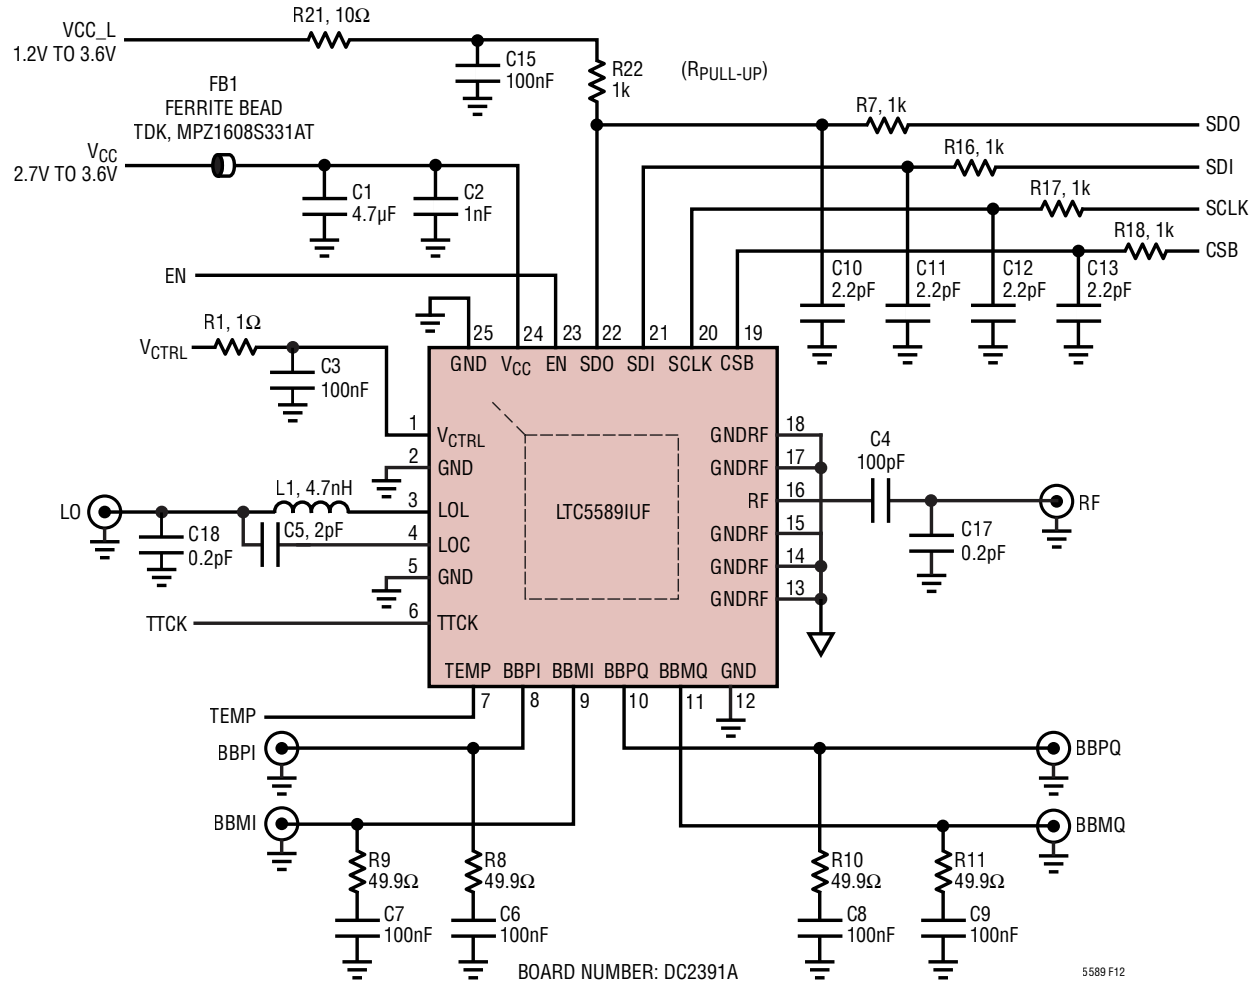
\includegraphics[width=0.7\linewidth]{figs/ch3_LTC5589_application.png}
    \caption{Recommended application circuit for the LTC5589 Modulator \cite{LTC5589}}
    \label{fig:ch3_LTC5589_application.png}
\end{figure}

\par Because of this, for our circuit, pins 19 through 22 will be grounded, as the datasheet warns that, for applications where \ac{spi} is not used, the pins must not be left floating.

\par There is also the fact that the modulator will not be digitally controlled. We are interested only in setting it up and not having to worry about it anymore. As such, we will be changing some other pin configurations in order to have the LTC5589 working as the project requires.

\par The pin responsible for the Variable Gain Control Input, $V_{CTRL}$ (pin 1), is going to be connected to $3.3\:\si{V}$, in order to set the modulator to operate with the maximum gain factor that it can.

\par As we have no interest in measuring the temperature of the modulator, pins 6 and 7, TTCK and TEMP respectively, will both be connected to ground. The datasheet explicitly warns against leaving pin 6 floating.

\par Pin 23 would allow us to control whether or not the component is completely on. For the purpose of this project, the modulator will always work properly and, as such, will be directly connected to $3.3\:\si{V}$. Once again, it is advised that the pin should not be left floating.

\subsubsection{Baseband signals \ac{i} and \ac{q}}
\par The LTC5589 quadrature modulator has some particular requirements when it comes to supplying it with appropriate \ac{i} and \ac{q} components. It mentions that the signals must be supplied to the device as differential inputs to the BBPI, BBMI pins for the \ac{i} signal and BBPQ, BBMQ for the \ac{q} signal. These signals must have a common mode level of $1.4\:\si{V}$ up to $2.0\:\si{V}$, as specified by the datasheet.

\par In order to interface the device with the signals for the modulator, a circuit block that would convert these single ended signals into differential signals had to be designed. 

\par For this circuit, two OpAmps were used, in a configuration equal to the one seen in Figure \ref{fig:ch3_LTC5589interfaceCirc.png}, which is explained in a Texas Instruments's application note. The OpAmps chosen for this circuit were OPA2607IDR from Texas Instruments.

\begin{figure}[H]
    \vspace*{0cm}
    \centering
    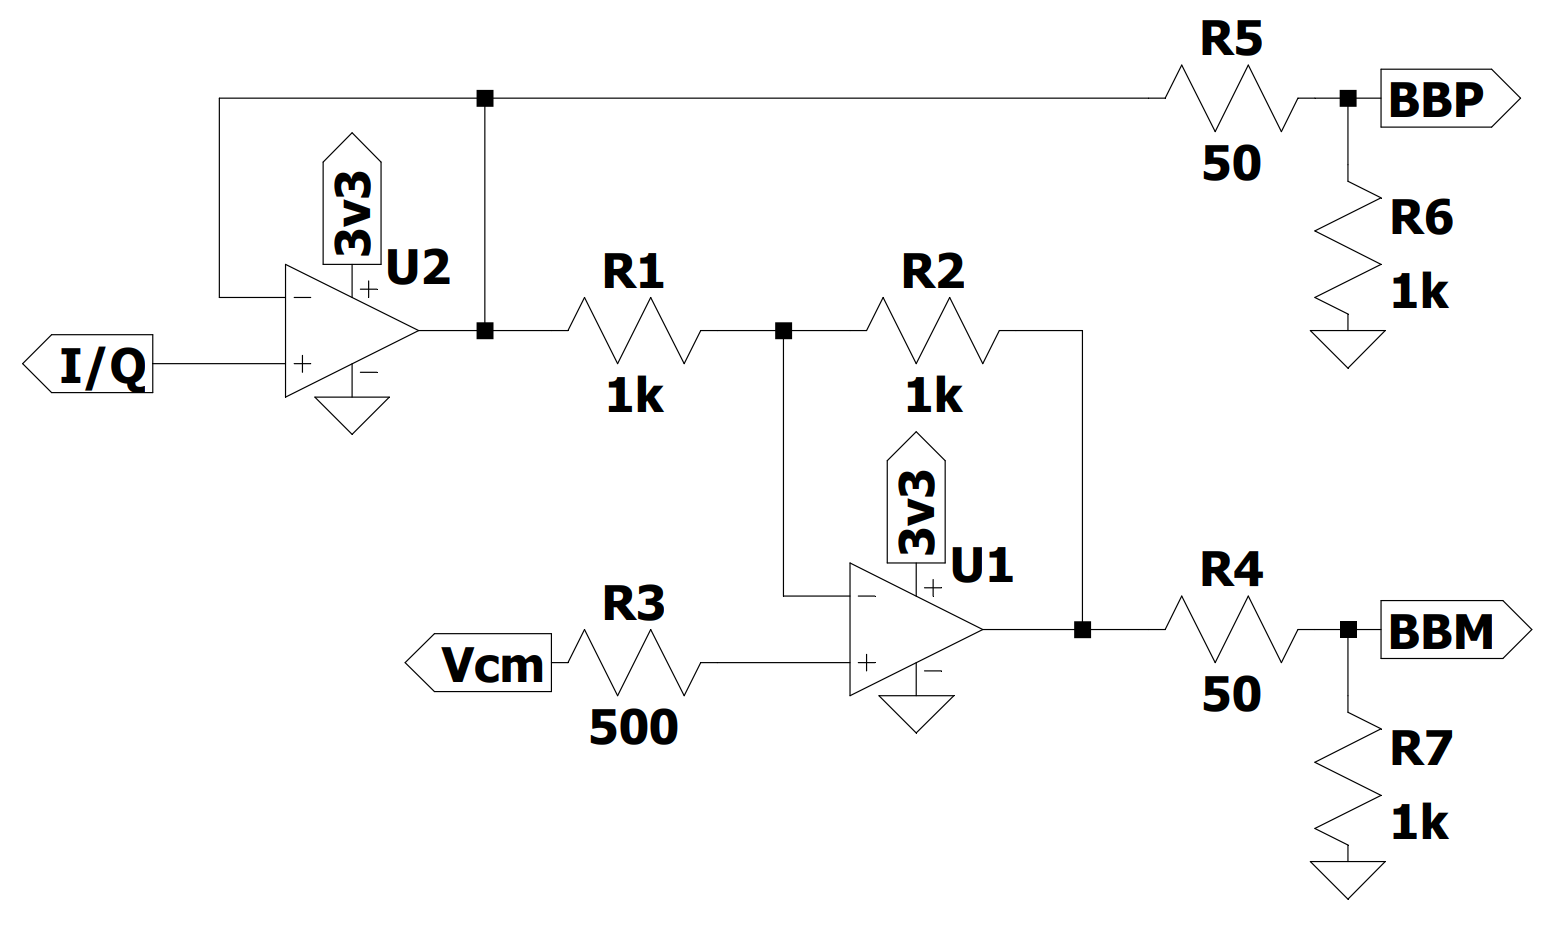
\includegraphics[width=0.7\linewidth]{figs/ch3_LTC5589interfaceCirc.png}
    \caption{Circuit block to interface \ac{iq} signals: single ended to differential}
    \label{fig:ch3_LTC5589interfaceCirc.png}
\end{figure}

\par For this circuit block, a simulation is performed using LTSpice, Analog Devices SPICE simulator software, that results in the output seen in Figure \ref{fig:ch3_LTC5589interfacePlot}.

\begin{figure}[H]
    \vspace*{0cm}
    \centering
    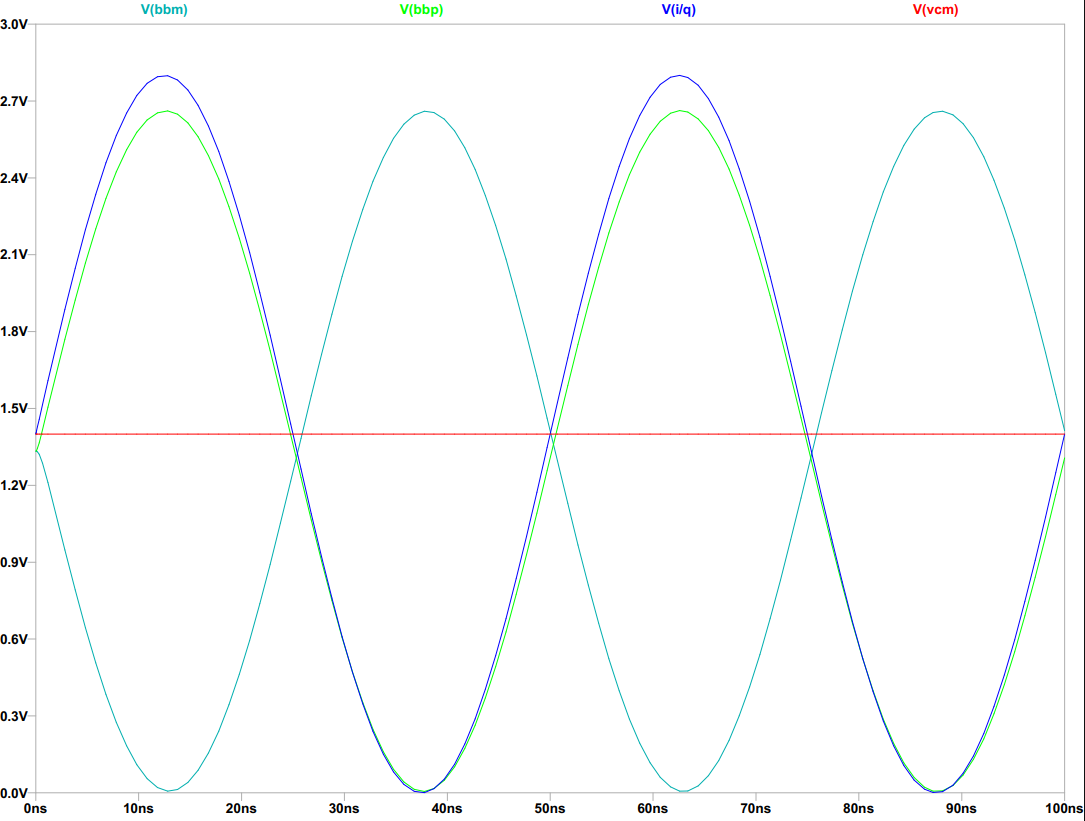
\includegraphics[width=0.7\linewidth]{figs/ch3_LTC5589interfacePlot.png}
    \caption{Simulation results of the single ended to differential converter}
    \label{fig:ch3_LTC5589interfacePlot}
\end{figure}

\par There was always a focus on procuring resistors, inductors, and capacitors capable suitable for operating at the frequencies to which they would be subject. This way we would not have to worry about undesirable behaviors that could be caused by parasitic characteristics of each component.

\subsection{Buck Converter}
\par In order to properly design this section of the circuit, the datasheet of the MC33063ADR section referring to this type of converter was closely followed.

\par We needed to develop a $28\:\si{V}$ to $3.3\:\si{V}$ buck converter. According to the datasheet we first had to define some design parameters for the circuit. 

\begin{itemize}
    \item $V_{SAT} = 0.45\:\si{V}$ for the saturation of the switch;
    \item $V_{F} = 0.45\:\si{V}$ for the forward voltage drop of the retifier;
    \item $I_{O} = 0.5\:\si{A}$ as maximum output current;
    \item $f_{MIN} = 11\:\si{KHz}$ for the minimum frequency at which the circuit would operate;
    \item $V_{R} = 0.05\:\si{V}$ for the maximum peak-to-peak ripple voltage for the output
\end{itemize}

\par Afterwards, we could calculate several values for several components that would allow the Buck converter to operate as we wanted. These values are registered in the following list of external components shown in Figure \ref{fig:ch3_BuckConf.png}.

\begin{itemize}
    \item $C_{T} = 487\:\si{pF}$
    \item $R_{SC} = 0.15\:\si{\Omega}$
    \item $L_{MIN} = 148 \:\si{\mu H}$
    \item $C_{O} = 455 \:\si{\mu F}$
\end{itemize}

\par As these values are not necessarily easy to obtain, as they are not in any common series of components, some compromises had to be made, without detracting from the overall performance of the Buck converter. As such, the components that were used for the project were

\begin{itemize}
    \item $C_{T} = 470\:\si{pF}$
    \item $R_{SC} = 0.33\:\si{\Omega}$
    \item $L_{MIN} = 220\:\si{\mu H}$
    \item $C_{O} = 470\:\si{\mu F}$
\end{itemize}

\par The datasheet also mentions the possibility of adding a filter at the output of the Buck converter. For the project that was being designed, it made sense to use one, as we did not want any undesirable fluctuations of the output voltage. A LC filter was added, with an inductor of $L = 1\:\si{\mu H}$ and a capacitor of $C = 100\:\si{\mu F}$.

\par Two resistors are used to set the desired output voltage, $V_{O}$. To calculate them we can use Equation \ref{ch3_buckResistors}.

\begin{equation}
    \label{ch3_buckResistors}
    V_{O} = 1.25\cdot\left(1+\frac{R2}{R1}\right)
\end{equation}

\par In order to find what was the better pair of values for these resistors, we can try an iterative process until we find two of these values that belong to a series of resistance or are very close to these values. In the end we obtained these values such that $R2 = 1.8\:\si{K\Omega}$ and $R1 = 1.1\:\si{K\Omega}$.

\par The overall design for this block of the project can be seen in Figure \ref{fig:ch3_BuckConf.png}.

\begin{figure}[H]
    \vspace*{0cm}
    \centering
    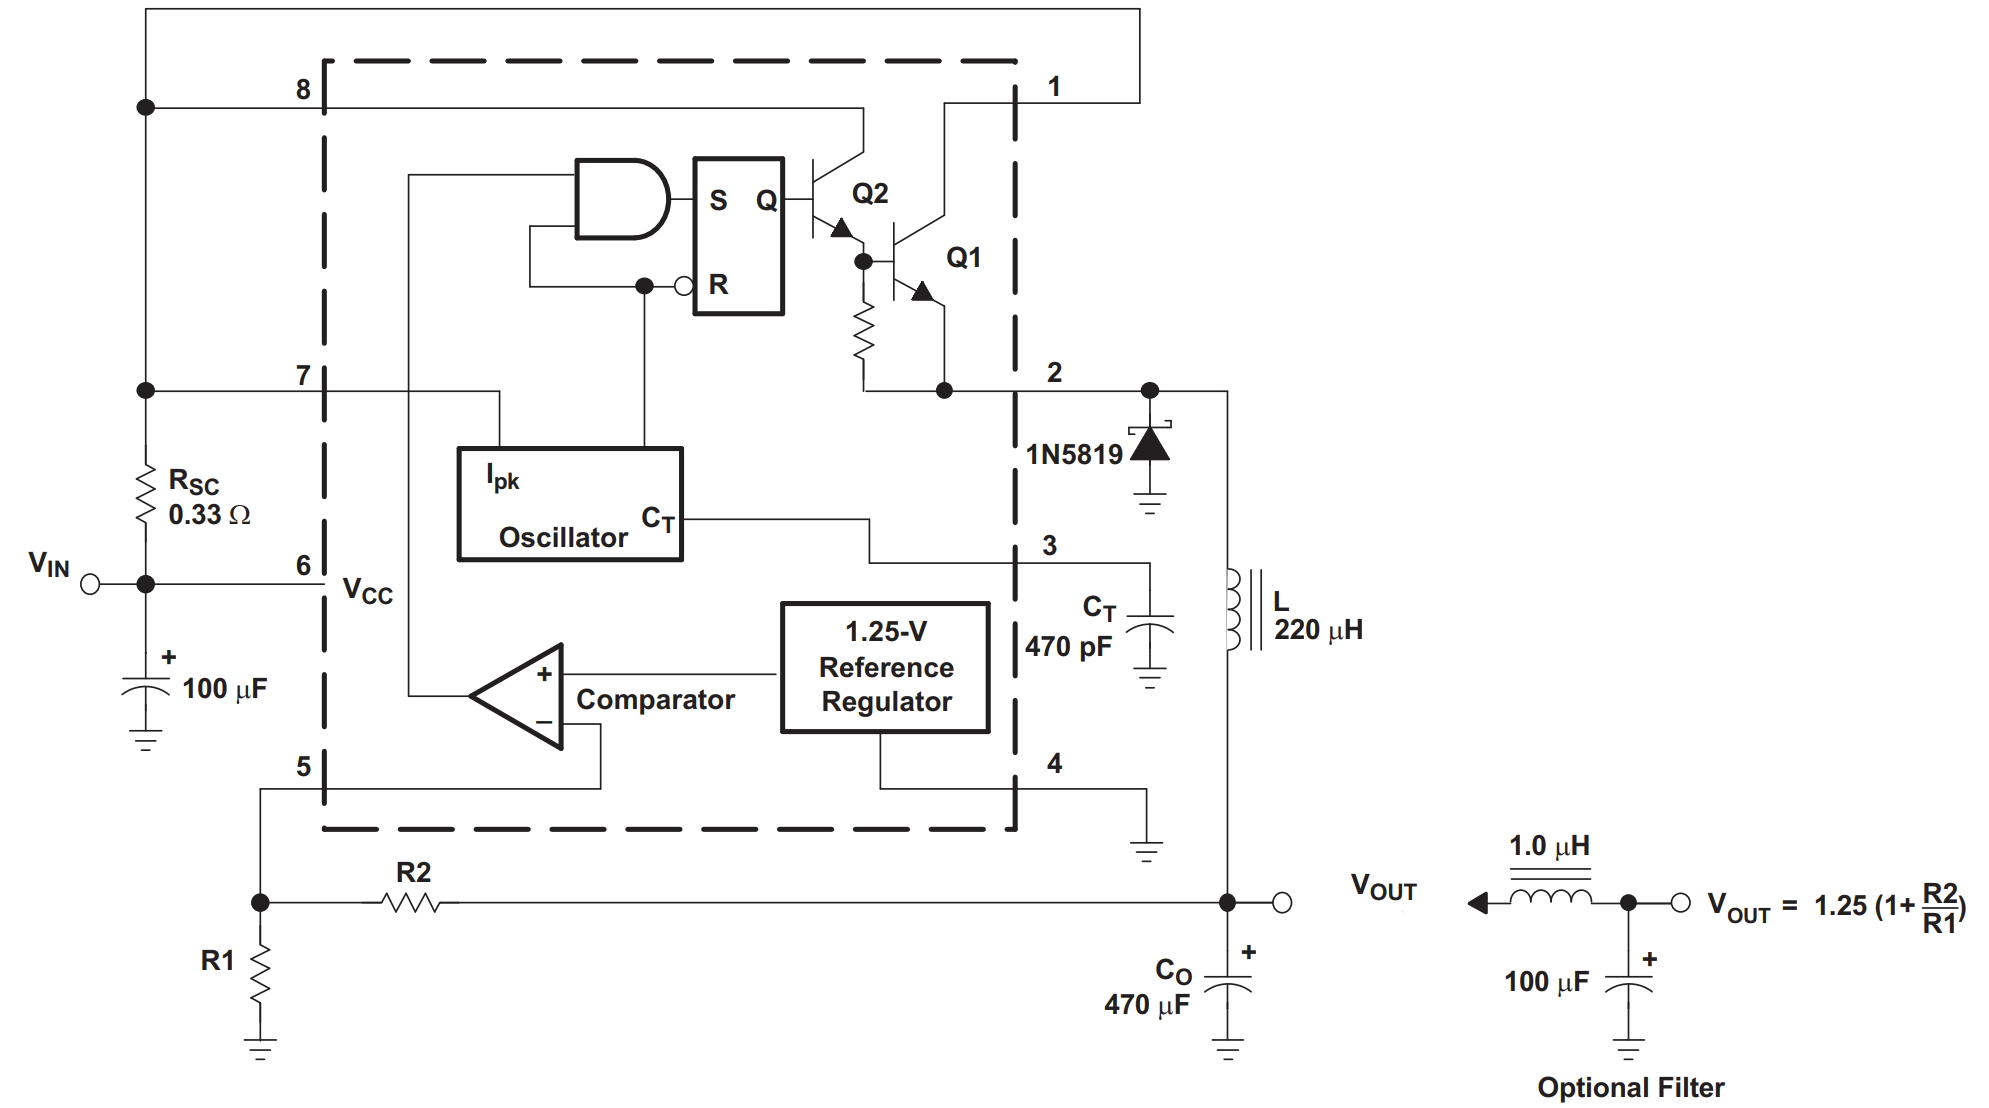
\includegraphics[width=0.9\linewidth]{figs/ch3_BuckConf.png}
    \caption{Buck converter design \cite{2004MC3x063ARegulators}}
    \label{fig:ch3_BuckConf.png}
\end{figure}

\subsection{Driver Amplifier}
\par In order to have the PGA-102r+ in working condition, as mentioned earlier, it needed to have a bias-tee associated with it. There were also two decoupling capacitors used for this component. The bias-tee was designed and simulated within with Keysight's PathWave Advanced Design System.

\par Using the s-parameter files made available by Mini-Circuits for the driver amplifier, we arrived at the following circuit, which is shown in Figure \ref{fig:ch3_PGAbiastee.png}.

\begin{figure}[H]
    \vspace*{0cm}
    \centering
    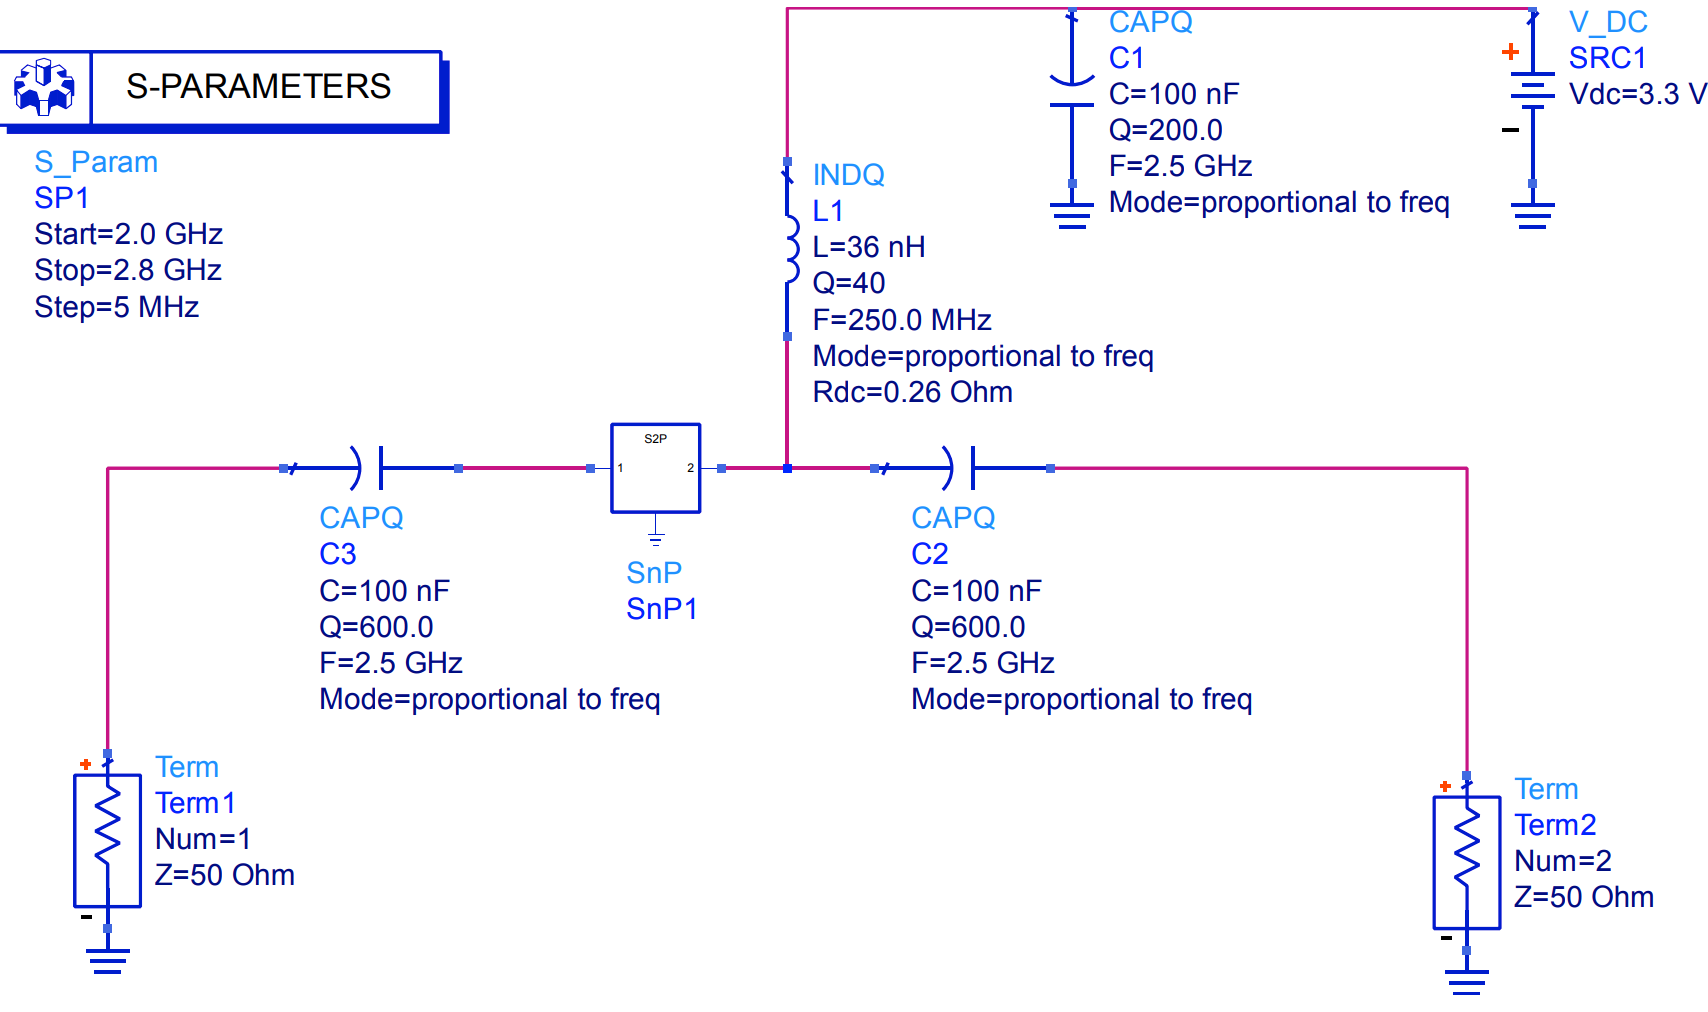
\includegraphics[width=0.9\linewidth]{figs/ch3_PGAbiastee.png}
    \caption{Circuit for the PGA-102+ bias-tee}
    \label{fig:ch3_PGAbiastee.png}
\end{figure}

\par The results obtained after the simulation can be seen in Figure \ref{fig:ch3_PGASim.png}. Here we can see the expected Gain, Input and Output Return Loss. These results are very similar to the expected results from the component datasheet that are shown in Figures \ref{fig:ch3_PGAGainTheo.png} and \ref{fig:ch3_PGAioRLtheo.png}. We are only interested in the results for a frequency of $2.4 \:\si{GHz}$, with a supply of $3.3 \:\si{V}$ and at room temperature.

\begin{figure}[H]
    \vspace*{0cm}
    \centering
    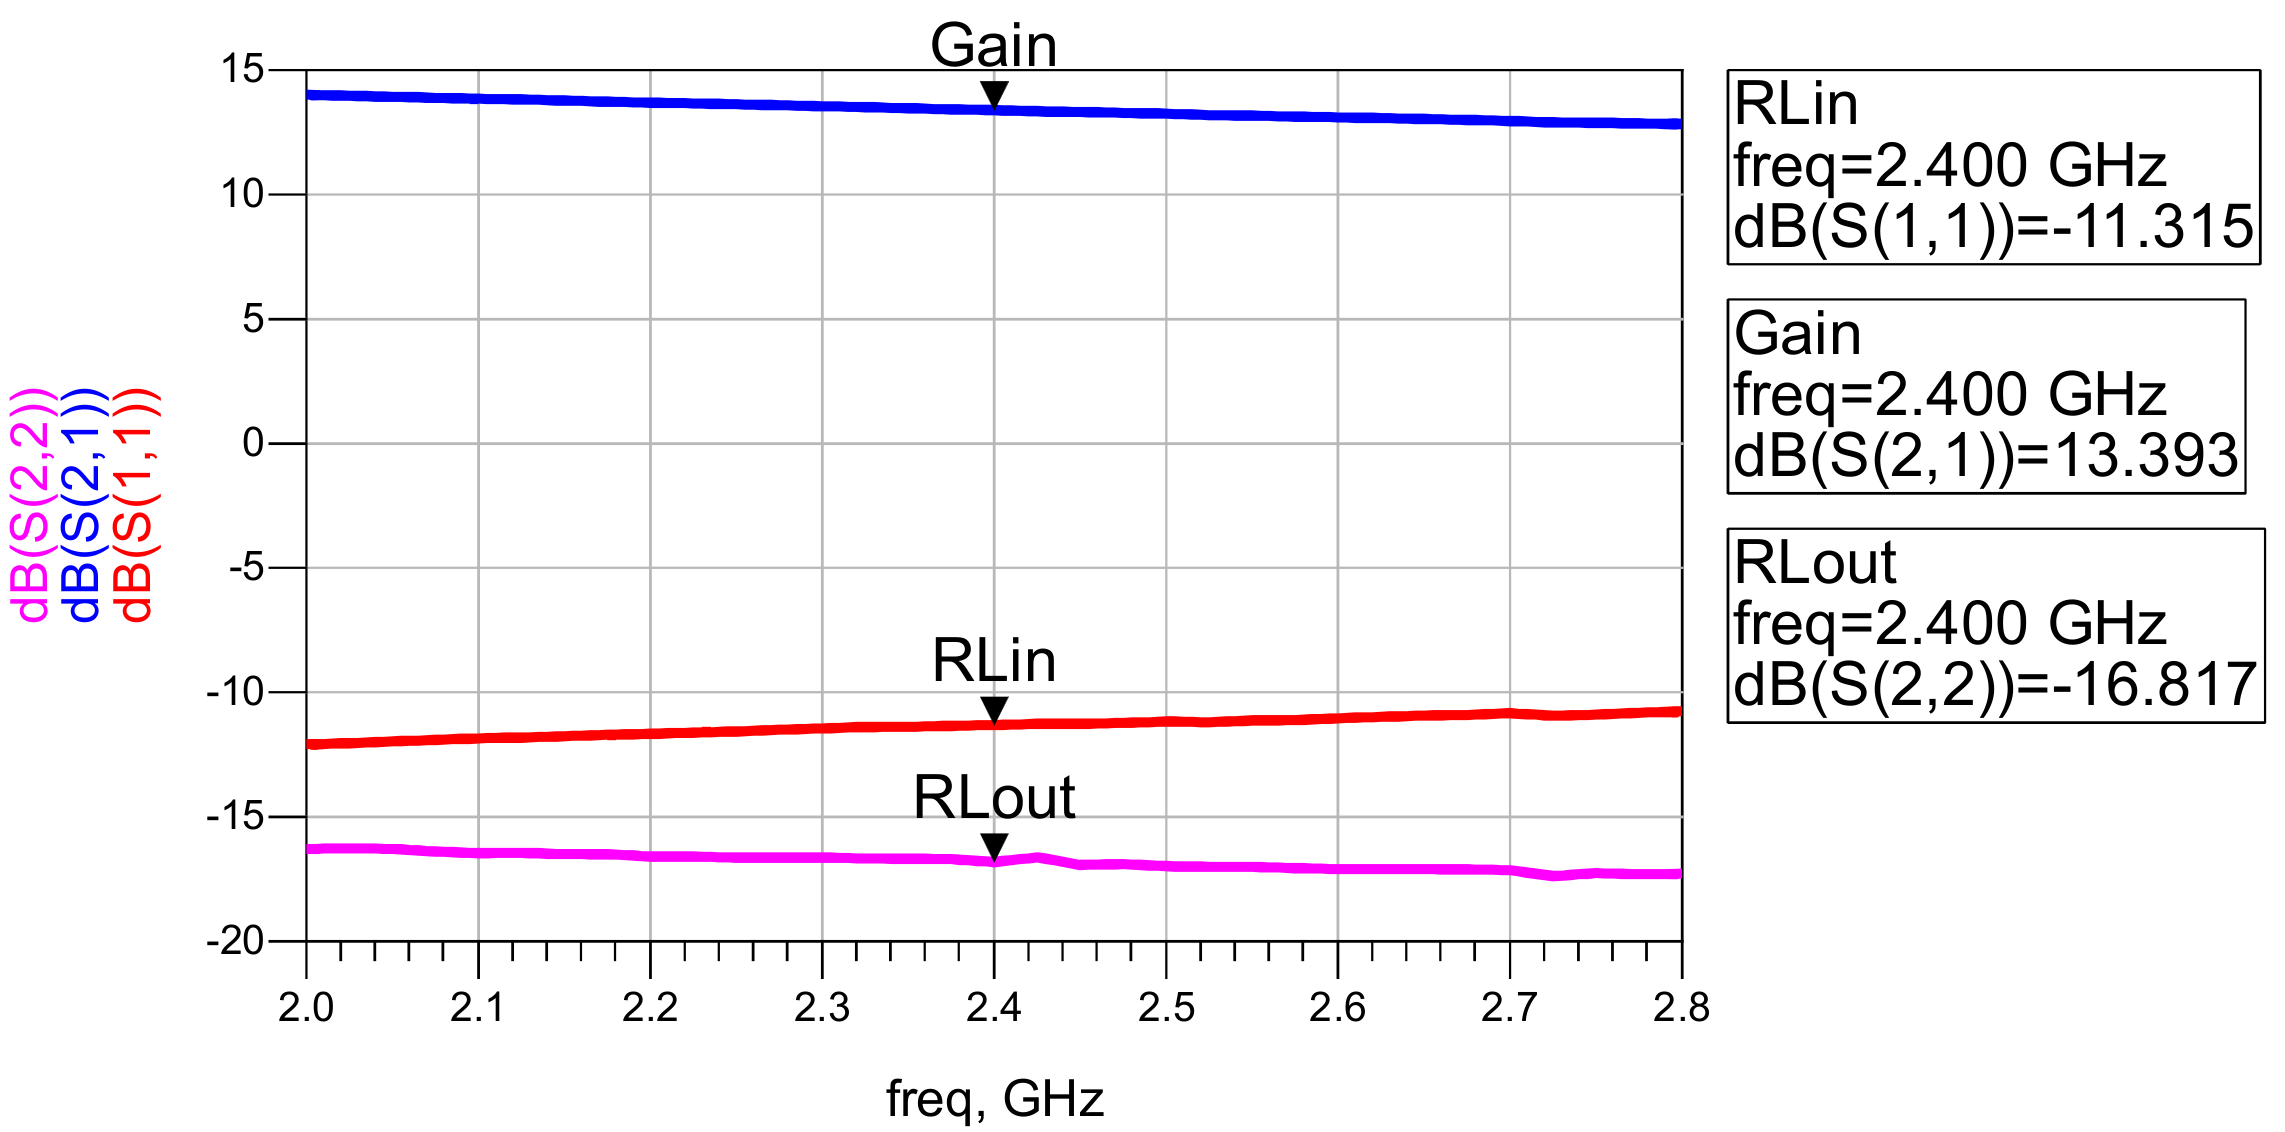
\includegraphics[width=0.9\linewidth]{figs/ch3_PGASim.png}
    \caption{Simulated results of the bias-tee developed}
    \label{fig:ch3_PGASim.png}
\end{figure}

\begin{figure}[H]
    \vspace*{0cm}
    \centering
    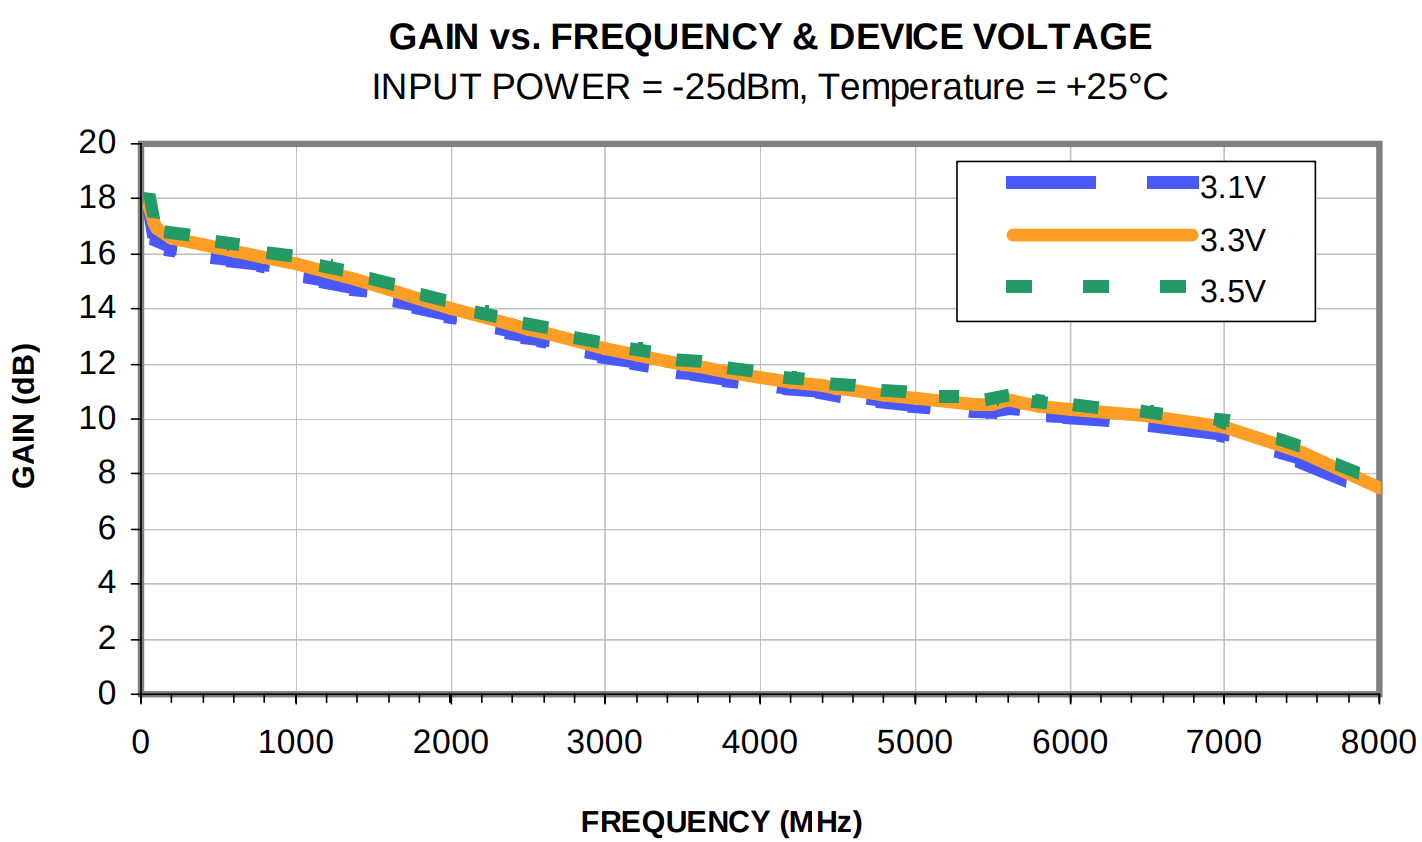
\includegraphics[width=0.9\linewidth]{figs/ch3_PGAGainTheo.png}
    \caption{Expected gain from the datasheet of PGA-102+ \cite{MonolithicPGA-102+}}
    \label{fig:ch3_PGAGainTheo.png}
\end{figure}

\begin{figure}[H]
    \vspace*{0cm}
    \centering
    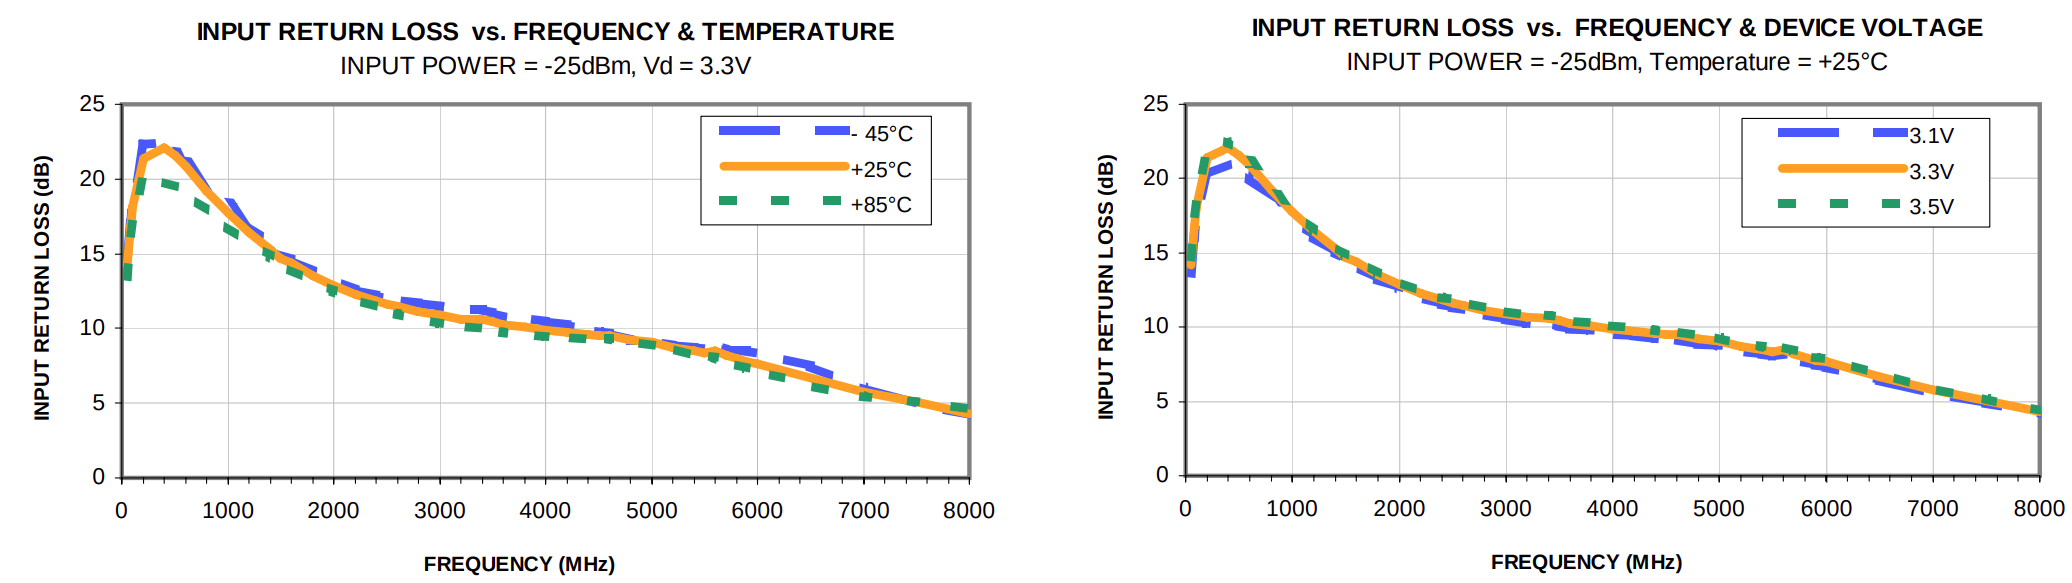
\includegraphics[width=0.9\linewidth]{figs/ch3_PGAioRLtheo.png}
    \caption{Input and Output Return Loss of the PGA-102+ driver amplifier \cite{MonolithicPGA-102+}}
    \label{fig:ch3_PGAioRLtheo.png}
\end{figure}

\par The results obtained were satisfactory and made us comfortable enough with them, so this design choice ended up being used for the project.

\subsection{\acl{pa}}
\par For the circuit assembly of the \ac{pa}, we tried to follow the the evaluation board layout on Figure \ref{fig:ch3_NPA1007eval.png} that is present on the datasheet of the NPA1007, as it was compliant with the majority of the specifications. The only specifications that this design did not respect was the ability to control the gate voltage with a potentiometer or having a circulator.

\begin{figure}[H]
    \vspace*{0cm}
    \centering
    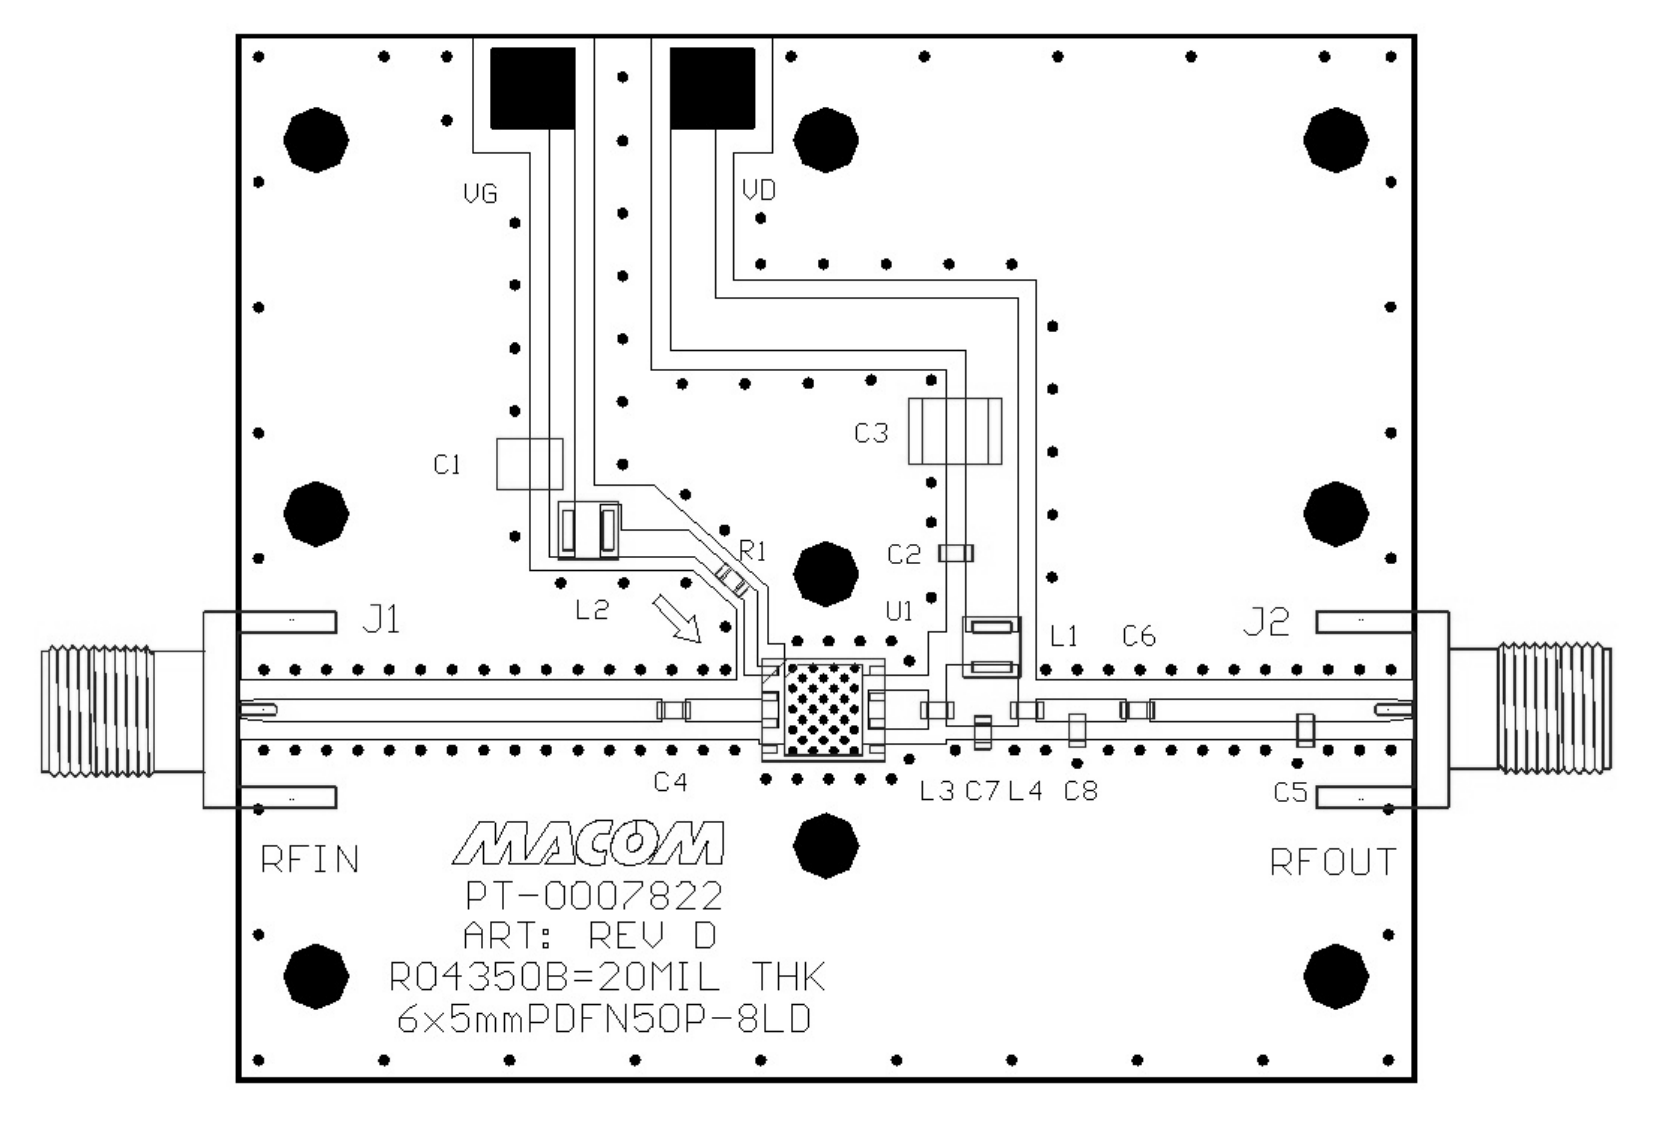
\includegraphics[width=0.9\linewidth]{figs/ch3_NPA1007eval.png}
    \caption{Suggested design for an Evaluation Board from MACOM's NPA1007 \cite{NPA1007}}
    \label{fig:ch3_NPA1007eval.png}
\end{figure}

\par The circuit schematic for the evaluation circuit can be better seen in Figure \ref{fig:ch3_NPA1007schematic.png}. The initial idea would be to utilize the components that are specified by the MACOM. Unfortunately, we were unable to acquire the specified capacitors C5, C7 and C8 sold by Passive Plus (PPI), and those had to be changed for ones that had similar characteristics.

\begin{figure}[H]
    \vspace*{0cm}
    \centering
    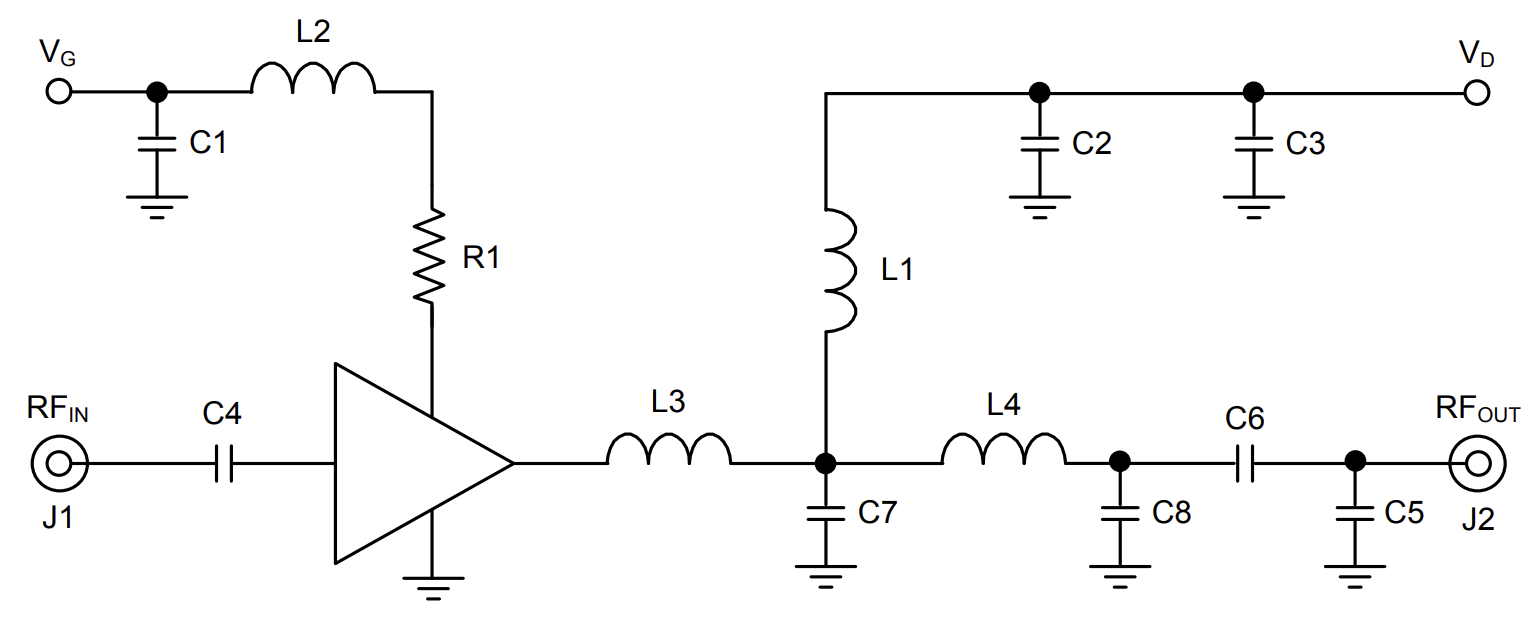
\includegraphics[width=0.9\linewidth]{figs/ch3_NPA1007schematic.png}
    \caption{Schematic for NPA1007 Evaluation Board \cite{NPA1007}}
    \label{fig:ch3_NPA1007schematic.png}
\end{figure}


\par In order to control the gate voltage, a potentiometer should be placed before C1. The chosen potentiometer was a $10\:\si{K\Omega}$, which should be placed as seen in Figure \ref{fig:ch3_NPA1007potentiometer.png}. Unfortunately, during the design of the \ac{pcb}, I mistakenly connected the potentiometer as shown in Figure \ref{fig:ch3_NPA1007potentiometerWRONG.png}. This error prevented the use of the potentiometer to set an adjustable fixed value for $V_{G}$ during the testing phase, as it was essentially a bypass of the potentiometer or the addition of a variable resistance in series with the proposed circuit, depending on how the potentiometer was configured. It made sense to simply bypass the potentiometer and control $V_{G}$ by varying the voltage set on a bench power supply.

\begin{figure}[H]
    \vspace*{0cm}
    \centering
    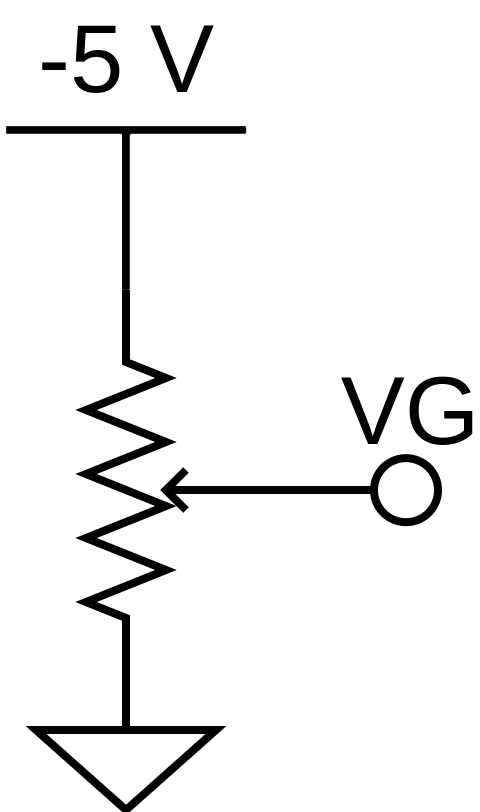
\includegraphics[width=0.12\linewidth]{figs/ch3_NPA1007potentiometer.png}
    \caption{Control of $V_{G}$ using a potentiometer corrected}
    \label{fig:ch3_NPA1007potentiometer.png}
\end{figure}

\begin{figure}[H]
    \vspace*{0cm}
    \centering
    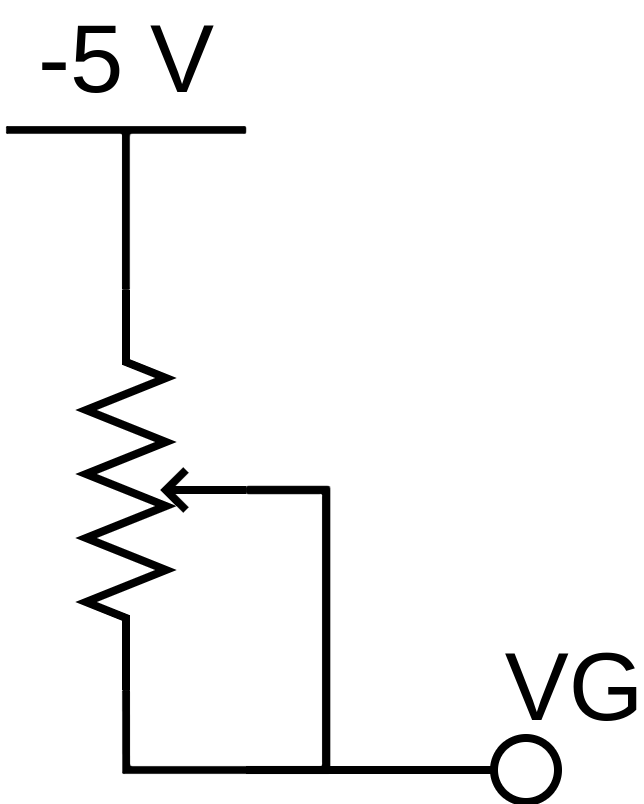
\includegraphics[width=0.15\linewidth]{figs/ch3_NPA1007potentiometerWRONG.png}
    \caption{Control of $V_{G}$ using a potentiometer, using a wrong solution}
    \label{fig:ch3_NPA1007potentiometerWRONG.png}
\end{figure}

\par It was attempted to acquire the models for this component to use in simulations on PathWave ADS, to evaluate the potential behavior of the project. The manufacturer was contacted via e-mail and failed to provide the necessary files to conduct these simulations. After discussing this with Professor Telmo Cunha, the idea of simulating the circuit was then abandoned.

\subsection{Design of the \ac{pcb}}
\par In order to design the \ac{pcb} we first have to understand the internal layout of the case for the circuit. Although the box has a tapering design and the top portion looks larger, from the inside the space is limited by four small plastic bosses where the lid fits in. This means that for a common rectangular \ac{pcb}, its dimensions must be so that it can fit within the space between these bosses. The internal dimensions of the case can be seen in Figure \ref{fig:ch3_CU-793-MBinternal.png} present in its datasheet.

\begin{figure}[H]
    \vspace*{0cm}
    \centering
    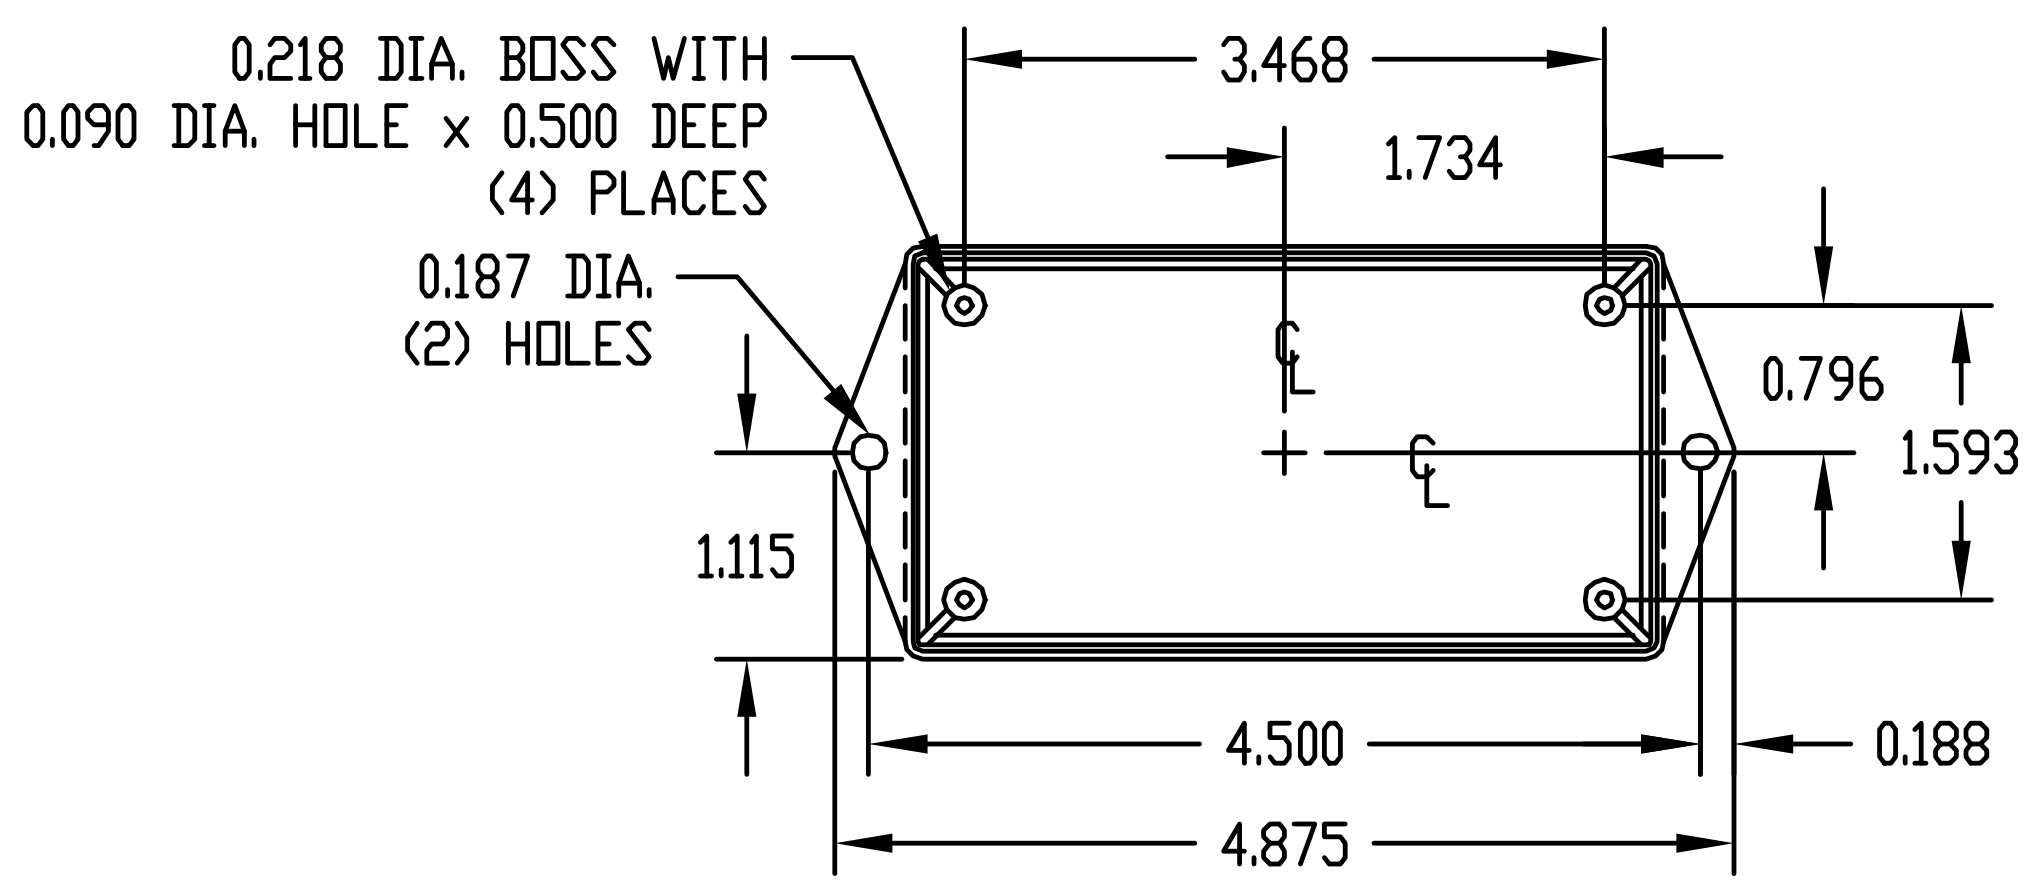
\includegraphics[width=0.7\linewidth]{figs/ch3_CU-793-MBinternal.png}
    \caption{Internal dimension of the CU-793-MB case \cite{UtiliboxCUR-793}}
    \label{fig:ch3_CU-793-MBinternal.png}
\end{figure}

\par So, in order to fit inside the case, our \ac{pcb} has to have a maximum width of $3.49 \:\si{cm}$ and length of $8.28 \:\si{cm}$. These restrictions made it impossible to fit the whole project in a single \ac{pcb} while trying to keep all components in the same layer, as the circuit that we planned to use for the \acl{pa} would occupy a significant portion of the layout. As such, it was devised that the circuit would be divided into two \ac{pcb}. The first, larger one would incorporate the majority of the components, and also all the inputs for the prototype. The second would be only for the \ac{pa} portion with its potentiometer and the circulator.

\par This meant that there had to be a way of maintaining the two different \ac{pcb} in position inside the case without touching each other. For this problem we figured that they could be kept separated if we used plastic washers placed between them. For this, we would leave three holes on each \ac{pcb}, where plastic studs could be inserted. The \ac{pcb} would be placed with their bottom layers facing each other and the top layers facing out. In this way there would be no chance of an accidental contact between their components, and we would not have any clearance problems related to component heights.

\par This approach is not without faults. There is now a need to pass both the $28\:\si{V}$, $-5\:\si{V}$, GND and the \ac{rf} signal that exits the driver amplifier to the second \ac{pcb}. For the DC signals and GND, common wires were used, in order to connect these signals. The driver would connect to the \ac{pa} via a small portion of coxial cable. Although the coaxial cable would already provide a suitable GND connection between both \ac{pcb}, we still used a wire connection.

\par In order to create the \ac{pcb}s, the footprints and models for the components when the manufacturer does not provide them, EAGLE from Autodesk was used. The bigger board has a length of $8\:\si{cm}$ and a width of $4\:\si{cm}$. This allows the board to sit inside the space created by the bosses. Although the width is bigger, this is by design as it does not allow movement of the board in at least one of the axes if it became loose. The final design of this board can be seen in Figure \ref{fig:ch3_PCBlayout1.png}.

\begin{figure}[H]
    \vspace*{0cm}
    \centering
    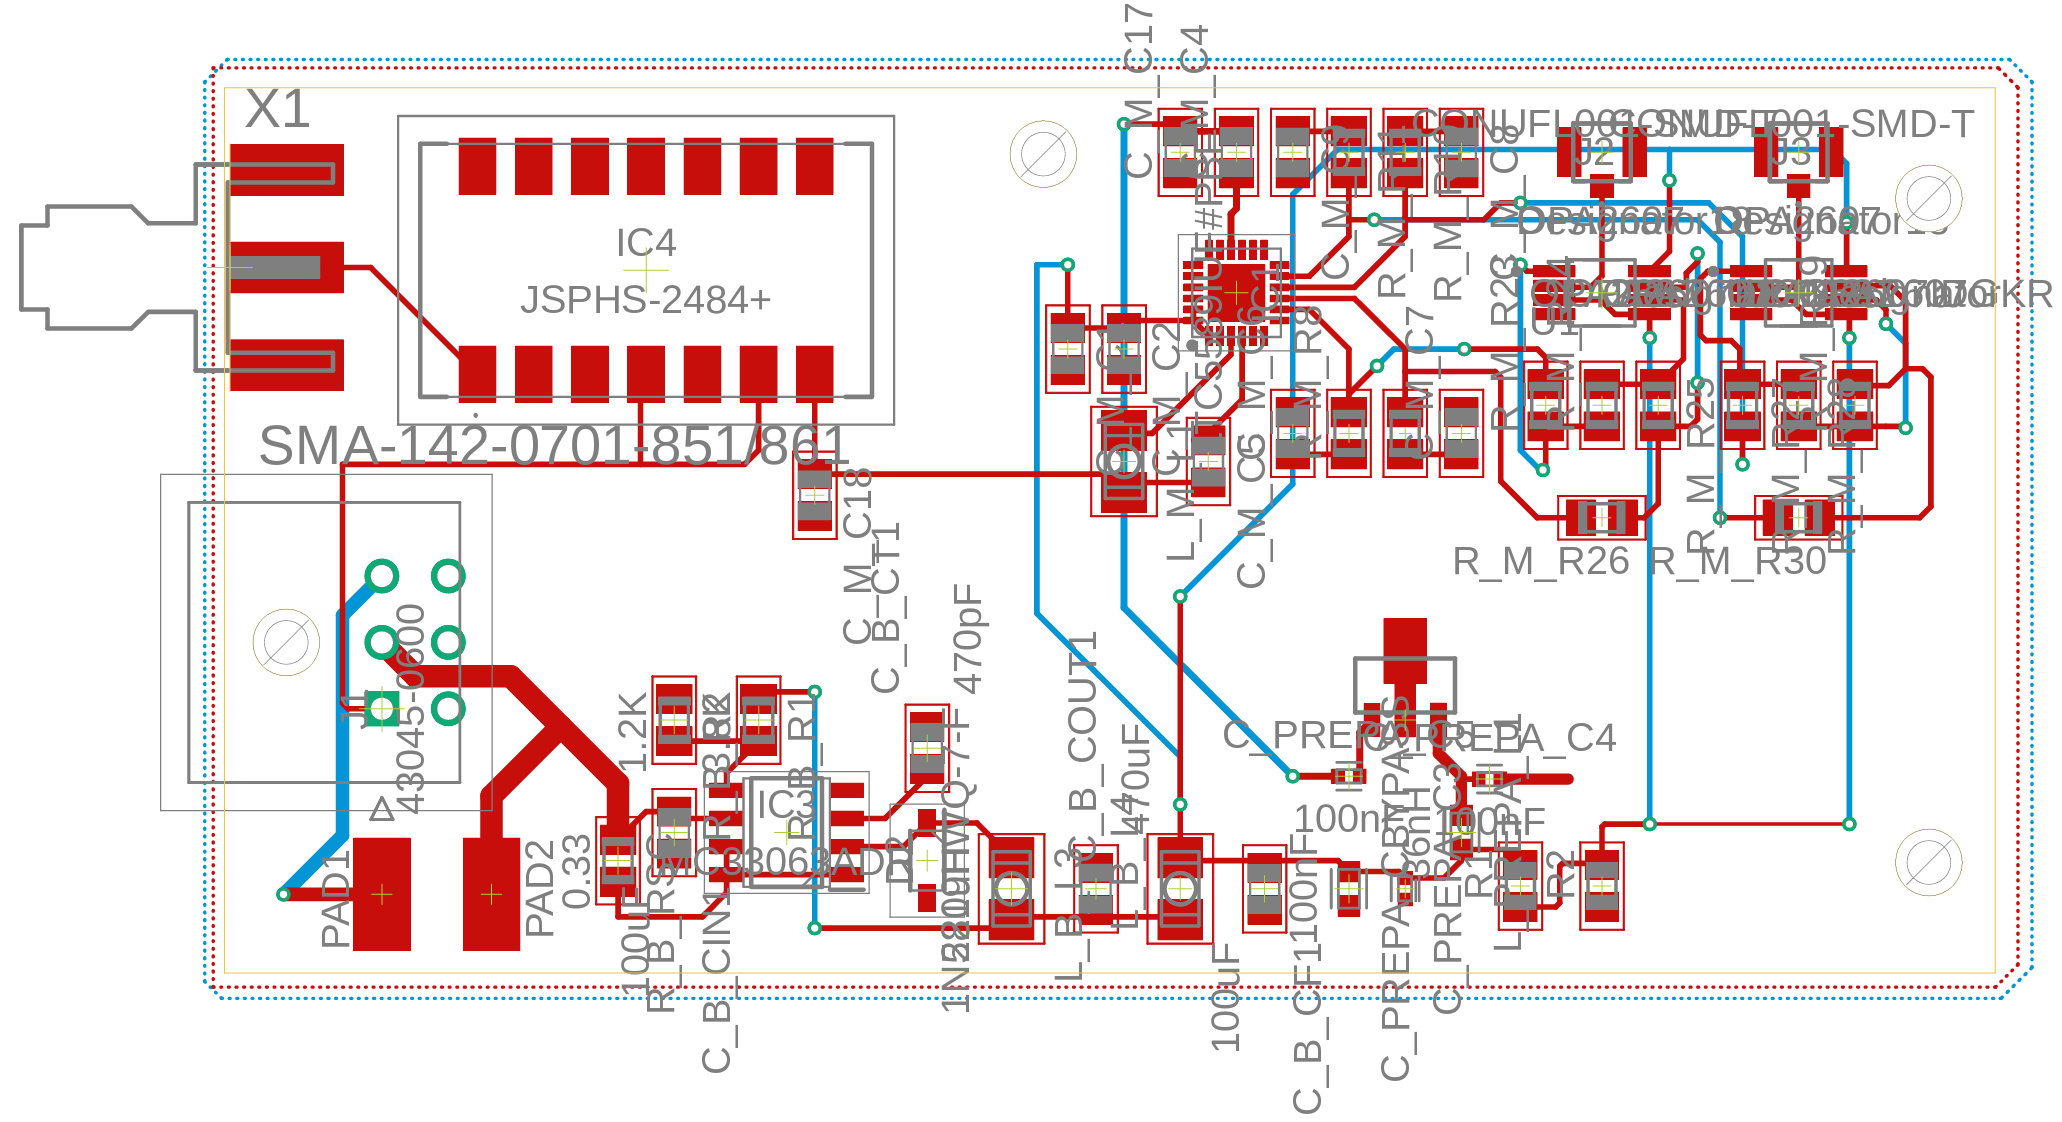
\includegraphics[width=0.8\linewidth]{figs/ch3_PCBlayout1.png}
    \caption{First \ac{pcb}}
    \label{fig:ch3_PCBlayout1.png}
\end{figure}

\par The three holes that were left in order to keep the board in position have a drill size of $3\:\si{mm}$ on EAGLE. These were positioned on both boards away so that they can be placed back-to-back. 

\par The \ac{pcb} for the \ac{pa} portion of the project has a smaller size, totaling $6\:\si{cm}$ in length and $4\:\si{cm}$ in width. On the second board, which contains the \ac{pa}, shown in Figure \ref{fig:ch3_PCBlayout1.png} we also added several through-hole vias that connect both sides of the board. This helps to distribute the heat that can be generated during operation. It should be noted, once again, that the connections to the potentiometer are wrong. This has been addressed earlier in the document.

\begin{figure}[H]
    \vspace*{0cm}
    \centering
    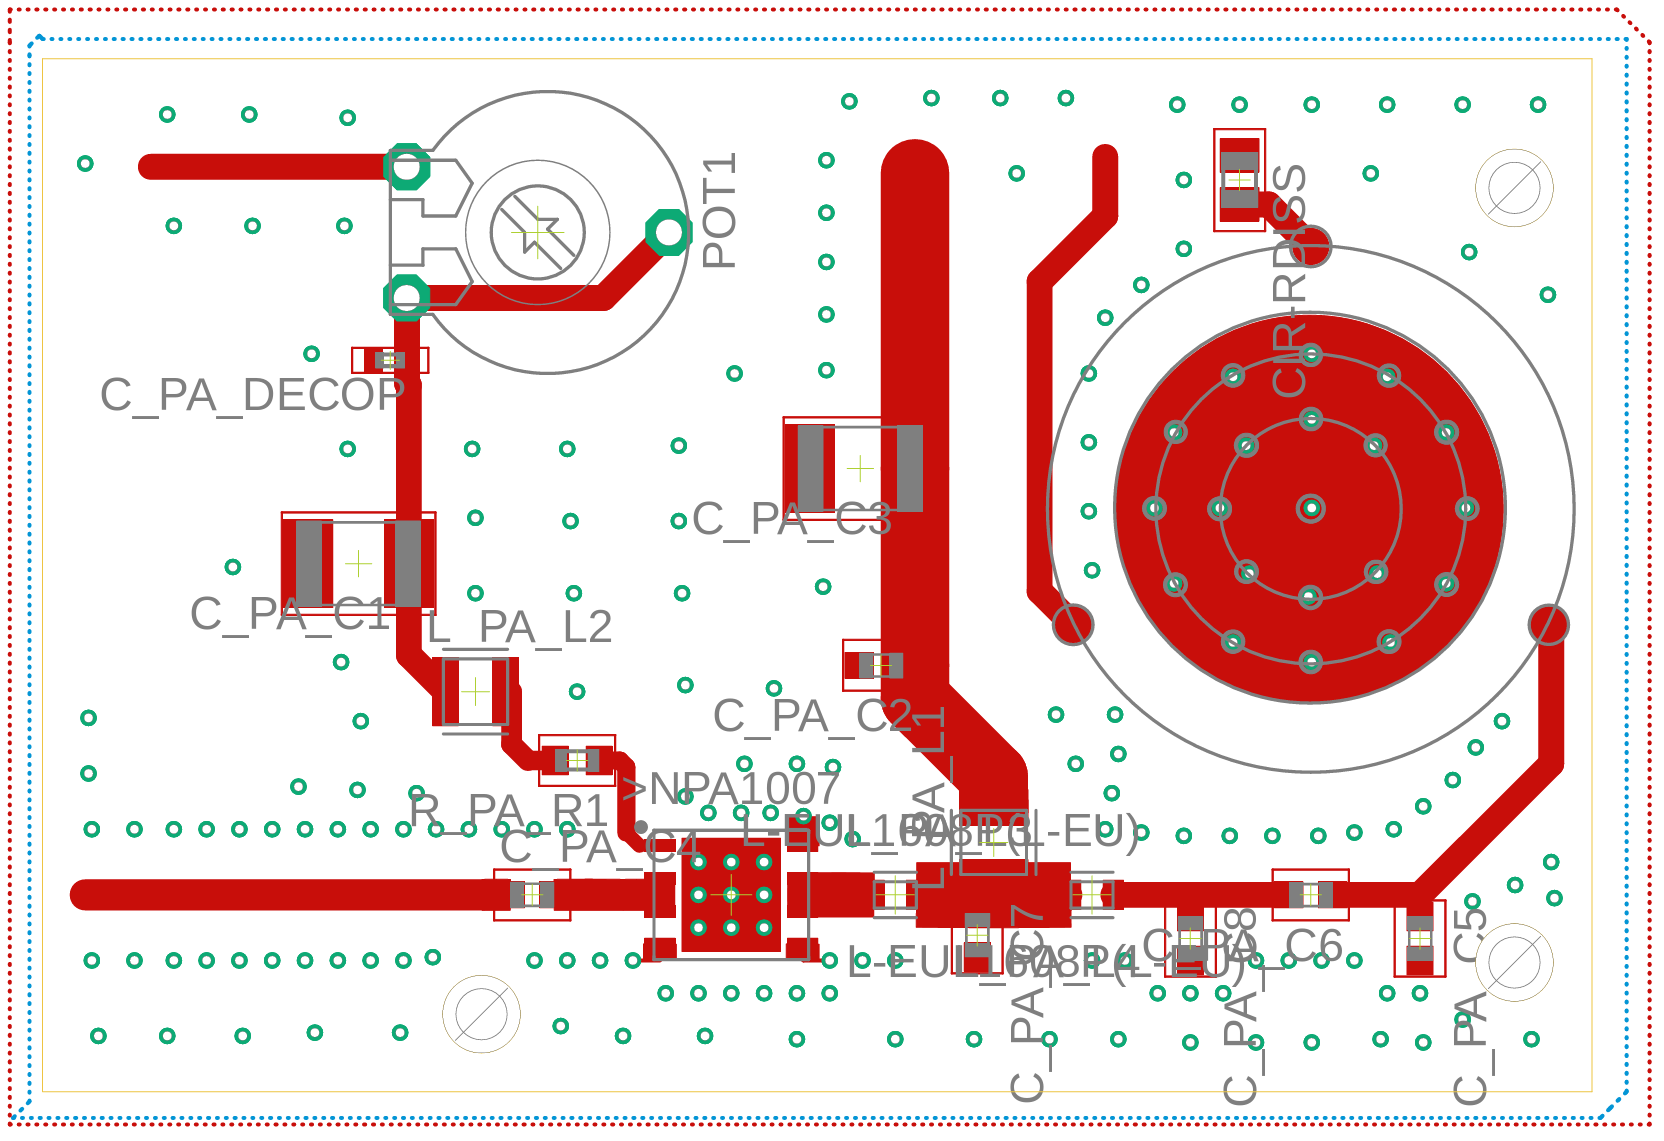
\includegraphics[width=0.8\linewidth]{figs/ch3_PCBlayout2.png}
    \caption{Second \ac{pcb}}
    \label{fig:ch3_PCBlayout2.png}
\end{figure}

\par It should be added that, although not entirely obvious from Figures \ref{fig:ch3_PCBlayout1.png} and \ref{fig:ch3_PCBlayout2.png}, both \ac{pcb} designs contain copper pours on the top and bottom layers. These are connected directly to GND.

\section{Spiral Antenna Design}
\par These types of antenna are characterized by their ability to have a consistence impedance and radiation pattern across a broad range of frequencies \cite{ConstantineA.Balanis2016AntennaDesign}. These antennas can have more than one arm, turning around itself forming a spiral. 

\par As they tend to generally have smaller sizes and respectable bandwidth, these can be used for application in broadband communication systems.

\par Spiral antennas operate by having resonance to different frequencies on different parts of the spiral, or spirals, that comprise them. Their design involves considering factors such as width of the arms or the spacing between them, the number of turns, and overall size of the antenna itself.

\par There are three main types of spiral antennas: archimedean, equiangular and logarithmic. For this project the focus was to create an archimedean type spiral antenna, having constant spacing between the two arms. In the end, after using Dassault Systems' CST Studio Suite to help with the design, our antenna was more of a logarithmic, with variable spacing between arms.

\par One characteristic of spiral antennas, and one that is a concern in this application, is that they radiate towards both sides. This means that if the antenna is in the front side of the box and radiates one of its two main lobes towards the intended location, there will inevitably be another main lobe in the opposite direction. 

\par This would not bode well for the operation of the array element, as it would be subject to a rather large power \ac{rf} signal potentially causing malfunction of the circuit and the equipment.

\par To prevent this problem, a box made of \ac{pcb} can be constructed around the antenna back, to protect the circuits behind it. This box will have a depth of around a quarter-wavelength of the desired carrier frequency. Theoretically, this depth would have been of $31.25\:\si{mm}$. This outer box is not connected to ground. This makes it so that any possible reflection would be canceled. 

\par In order to feed signal to the antenna, a front panel female SMA  connector is placed on the external part of the antenna box. To bridge the interior gap of the box, a small length of coaxial cable was used. This cable would then go through two small holes in the antenna arms to establish a connection.

\par The initial idea for the design of the antenna is explained by \citet{Caswell2002DesignSizes} on his PhD Thesis. Here, it is explained that the outer radius of the antenna, $R_{OUTER}$ can be calculated through (\ref{eq:ch3_outerRadius}). This dimension is directly related to the lowest frequency, $f_{LOW}$ of the desired range, because the lowest frequency at which the antenna resonates will have the longest wavelength.

\begin{equation}
    \label{eq:ch3_outerRadius}
    R_{OUTER} = \frac{c}{2\cdot f_{LOW}\cdot\pi}
\end{equation}

\par The inner radius of the antenna is calculated using Equation \ref{eq:ch3_innerRadius}. Because this length is related to the minimum wavelength at which the antenna will be able to resonate at, this sets the maximum frequency of the antenna, $f_{HIGH}$.

\begin{equation}
    \label{eq:ch3_innerRadius}
    R_{INNER} = \frac{c}{2\cdot f_{HIGH}\cdot\pi}
\end{equation}

\par The process of calculating the spacing between the arms, $S$, and the width of this arms, $W$, is explained by \cite{Caswell2002DesignSizes}. These two dimensions are the same for an archimedean antenna, as shown by Equation (\ref{eq:ch3_SandW}). In this equation $N$ refers to the number of turns of the antenna arms.

\begin{equation}
    \label{eq:ch3_SandW}
    s = w = \frac{r_{OUTER}-r_{INNER}}{4\cdot N}
\end{equation}

\par If we want to use these equations for an antenna with $N = 3.5$ that covers the interval from $1.8\:\si{GHz}$ to $5\:\si{GHz}$, we arrive at values for $R_{INNER} = 9.5\:\si{mm}$ and $R_{OUTER} = 2.7\:\si{cm}$, with a width and spacing of $1.18\:\si{mm}$.

\par We can fit the arms of such an antenna in a $5\:\si{cm}$ by $5\:\si{cm}$ square of substrate. The only problem is that we are going to have to angle this antenna so that the tips of its arms are at a corner rather than in the middle section of the square side. The substrate used for the antenna was RO4350B, while the one used for the box is FR-4.

\par The initial simulation performed in CST Studio for an antenna with these dimensions produced results that were not ideal for an antenna operating at a frequency of $2.4\:\si{GHz}$. Therefore, a process of iterative tuning of the parameters of the antenna was conducted within CST Studio.

\par In the end, we ended up with arms that were based on the lines with the equations that are shown on Figure \ref{fig:ch3_Spiral.png}.

\begin{figure}[H]
    \vspace*{0cm}
    \centering
    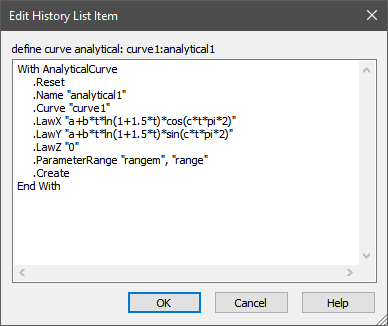
\includegraphics[width=0.5\linewidth]{figs/ch3_Spiral.png}
    \caption{Parameters for the line defining the arms}
    \label{fig:ch3_Spiral.png}
\end{figure}

\par After a long iterative optimization process, we arrived at an antenna that is shown in Figure \ref{fig:ch3_antenna.PNG}

\begin{figure}[H]
    \vspace*{0cm}
    \centering
    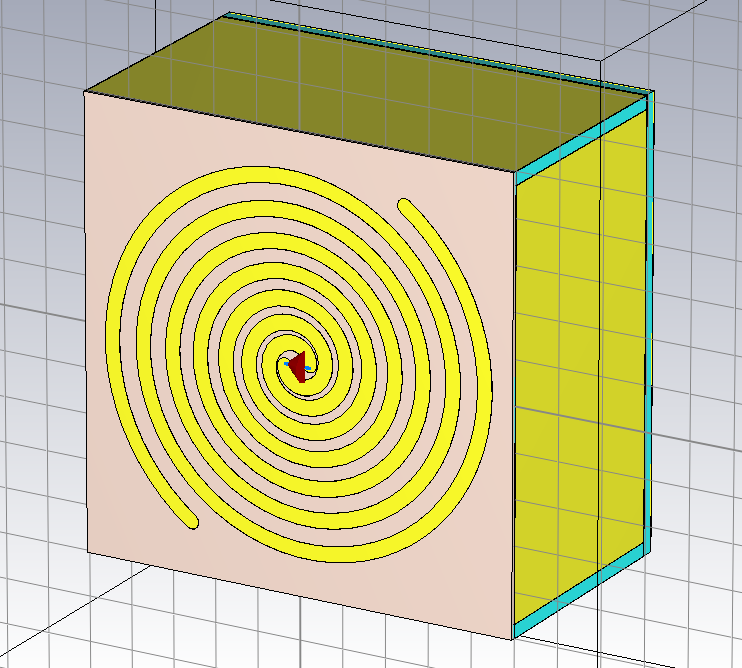
\includegraphics[width=0.5\linewidth]{figs/ch3_antenna.PNG}
    \caption{Antenna obtained on CST Studio}
    \label{fig:ch3_antenna.PNG}
\end{figure}

\par The dimensions of the antenna can be seen in Figure \ref{fig:ch3_parameter_list.PNG}. Here, "subsW" is the width of the antenna and "subsL" is its length. The parameters "subsTantenna" and "copperT" refer to characteristics of the substrate RO4350B, being both its thickness of the actual substrate and the thickness of the copper, respectively. The parameter "boxDepth" refers to the internal distance between the antenna and the opposite side of the box. The thickness of each side of the box is "subsT". All the other parameters help to control how the antenna's arms look. Both "rangem" and "a" help to indicate where the arms would start near the center. To control how closer the arms are to each other, "c" and "b" were used. To control the number of turns for each arm, we used the value of "range".

\begin{figure}[H]
    \vspace*{0cm}
    \centering
    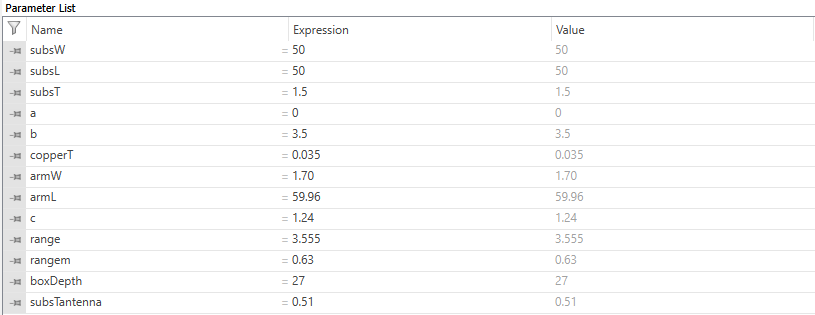
\includegraphics[width=0.9\linewidth]{figs/ch3_parameter_list.PNG}
    \caption{Parameter list for the construction and simulation of the antenna.}
    \label{fig:ch3_parameter_list.PNG}
\end{figure}

\par The obtained antenna performance can be seen in the next images. Figure \ref{fig:ch3_s11.png} shows the input reflection coefficient of the antenna. Although during the simulations performed on CST Studio the lowest value of S11 was not located at the frequency of $2.4\:\si{GHz}$, the antenna still had a decent reflection coefficient at that frequency. And with the certainty that when printed the physical antenna would not retain the same S11 parameter shown in CST Studio, we felt comfortable enough to use this design. 

\begin{figure}[H]
    \vspace*{0cm}
    \centering
    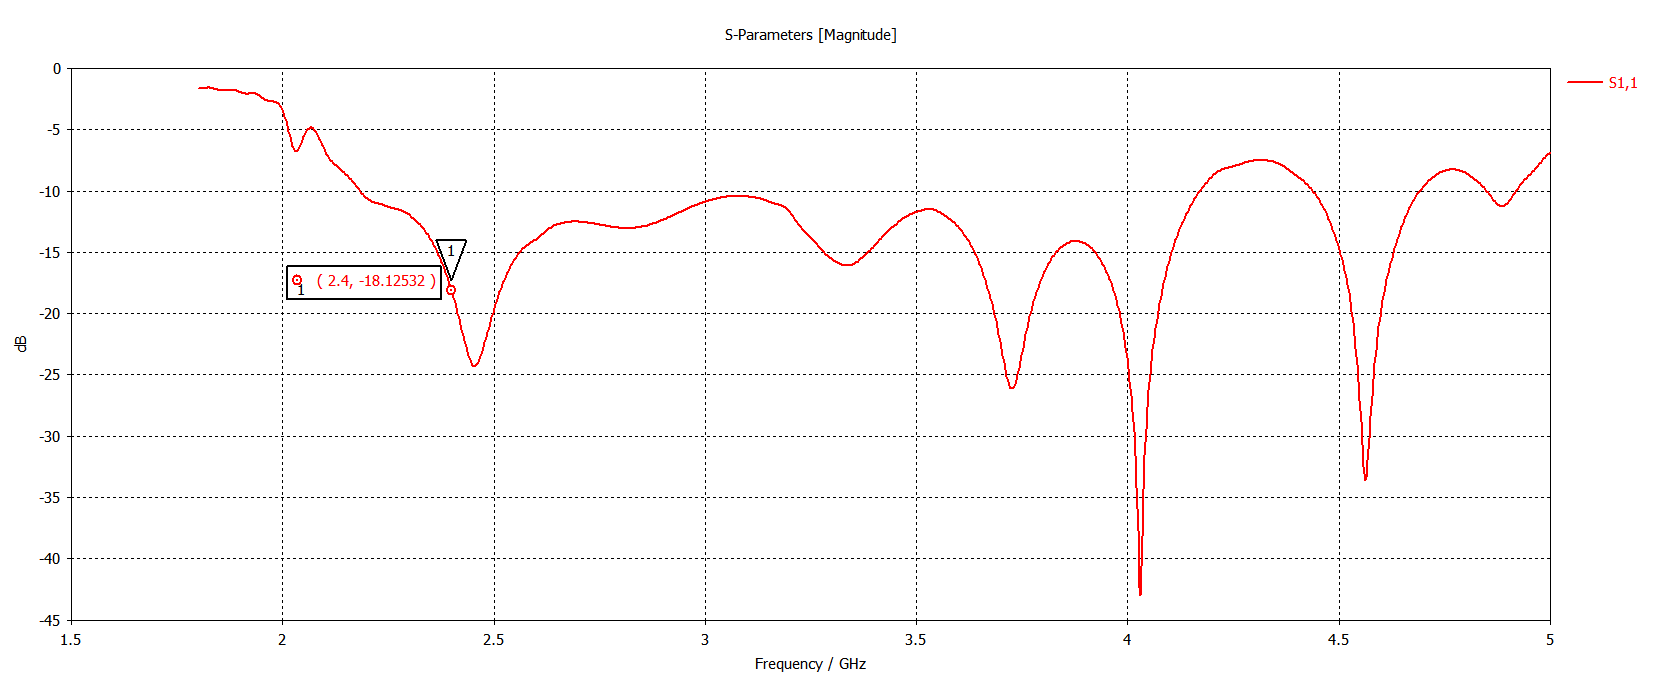
\includegraphics[width=0.9\linewidth]{figs/ch3_s11.png}
    \caption{VSWR of the antenna over frequency}
    \label{fig:ch3_s11.png}
\end{figure}

\par We can also observe the antenna's simulated VSWR in Figure \ref{fig:ch3_VSWR.png}, which is about $1.28$ for the desired frequency.

\begin{figure}[H]
    \vspace*{0cm}
    \centering
    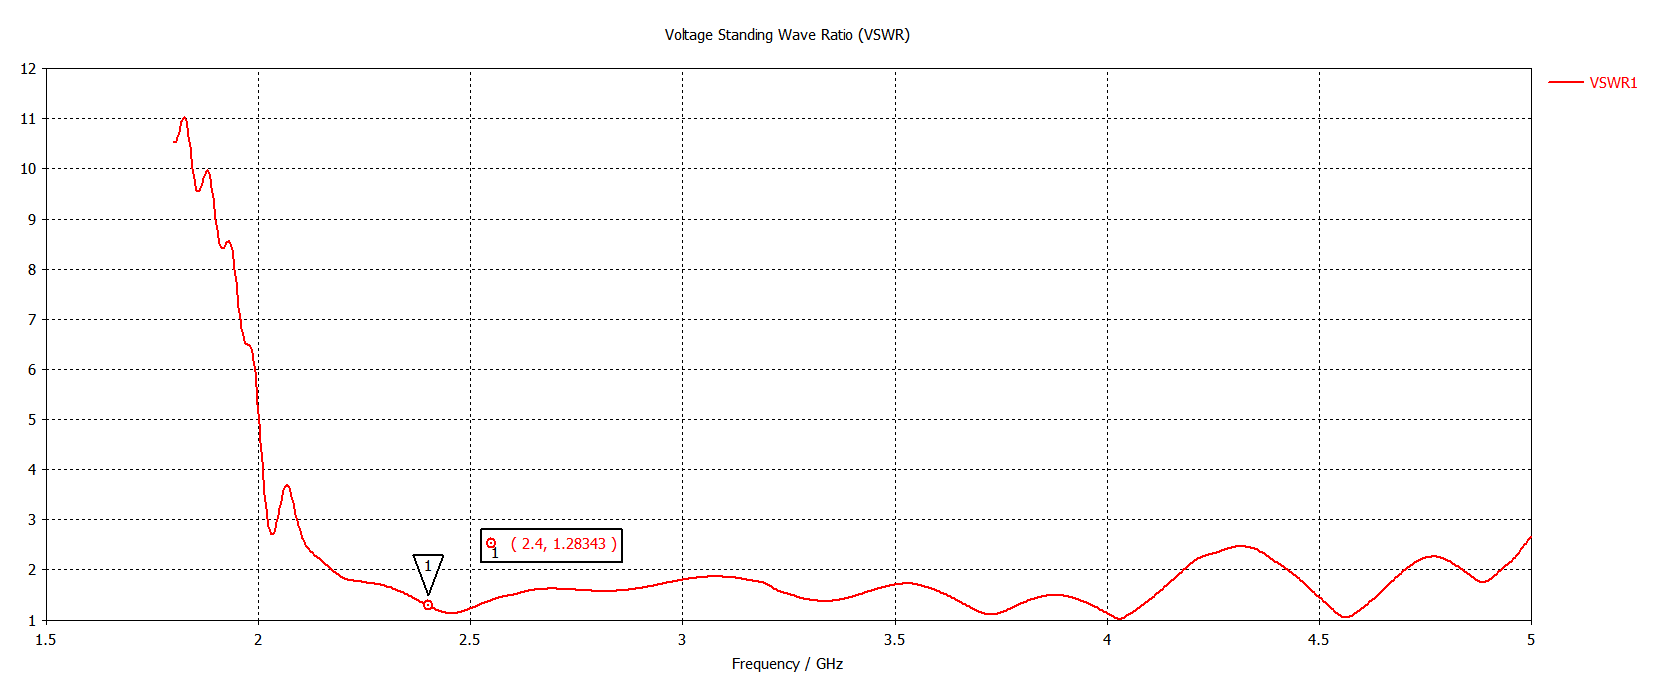
\includegraphics[width=0.9\linewidth]{figs/ch3_VSWR.png}
    \caption{VSWR of the antenna over frequency}
    \label{fig:ch3_VSWR.png}
\end{figure}

\par The Figures \ref{fig:ch3_farfield.PNG} and \ref{fig:ch3_farfieldBack.png} help visualize the form of the antenna radiation pattern. As we can see, the antenna does have good directivity coming in at $6.186\:\si{dBi}$ for the front, and being able to have a reduced value for the back. This helps understand better the effects of the box on the radiation pattern of the antenna.

\begin{figure}[H]
    \vspace*{0cm}
    \centering
    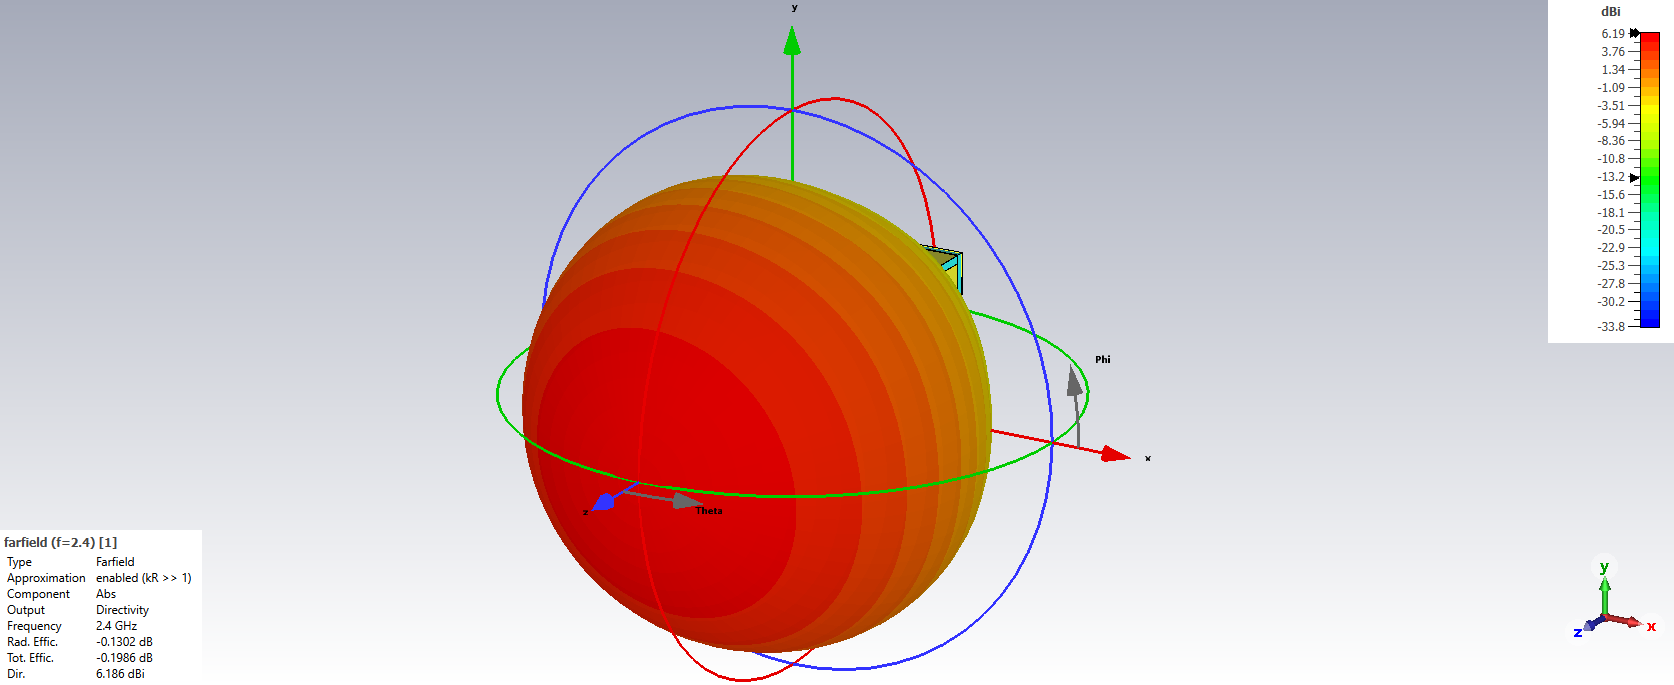
\includegraphics[width=0.9\linewidth]{figs/ch3_farfield.png}
    \caption{Front facing directivity}
    \label{fig:ch3_farfield.PNG}
\end{figure}

\begin{figure}[H]
    \vspace*{0cm}
    \centering
    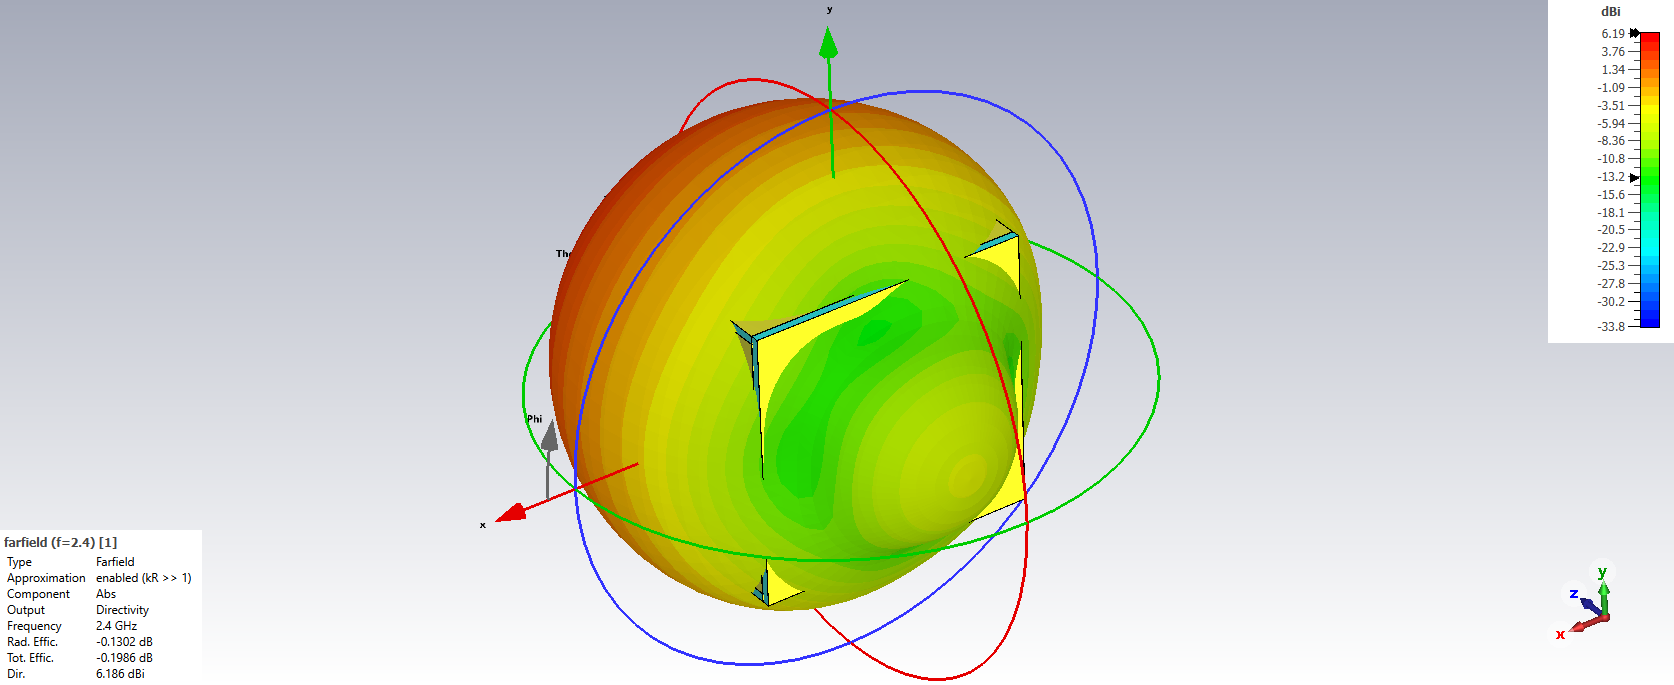
\includegraphics[width=0.9\linewidth]{figs/ch3_farfieldBack.png}
    \caption{Back facing directivity}
    \label{fig:ch3_farfieldBack.png}
\end{figure}

\par A better way to observe the farfield directivity of the antenna is through Figure \ref{fig:ch3_farfield1D.png}. Here, we can see the body of the antenna, as well as how it is radiating. We can also see that in simulation there is an offset of 2º on the main lobe direction of the antenna.

\begin{figure}[H]
    \vspace*{0cm}
    \centering
    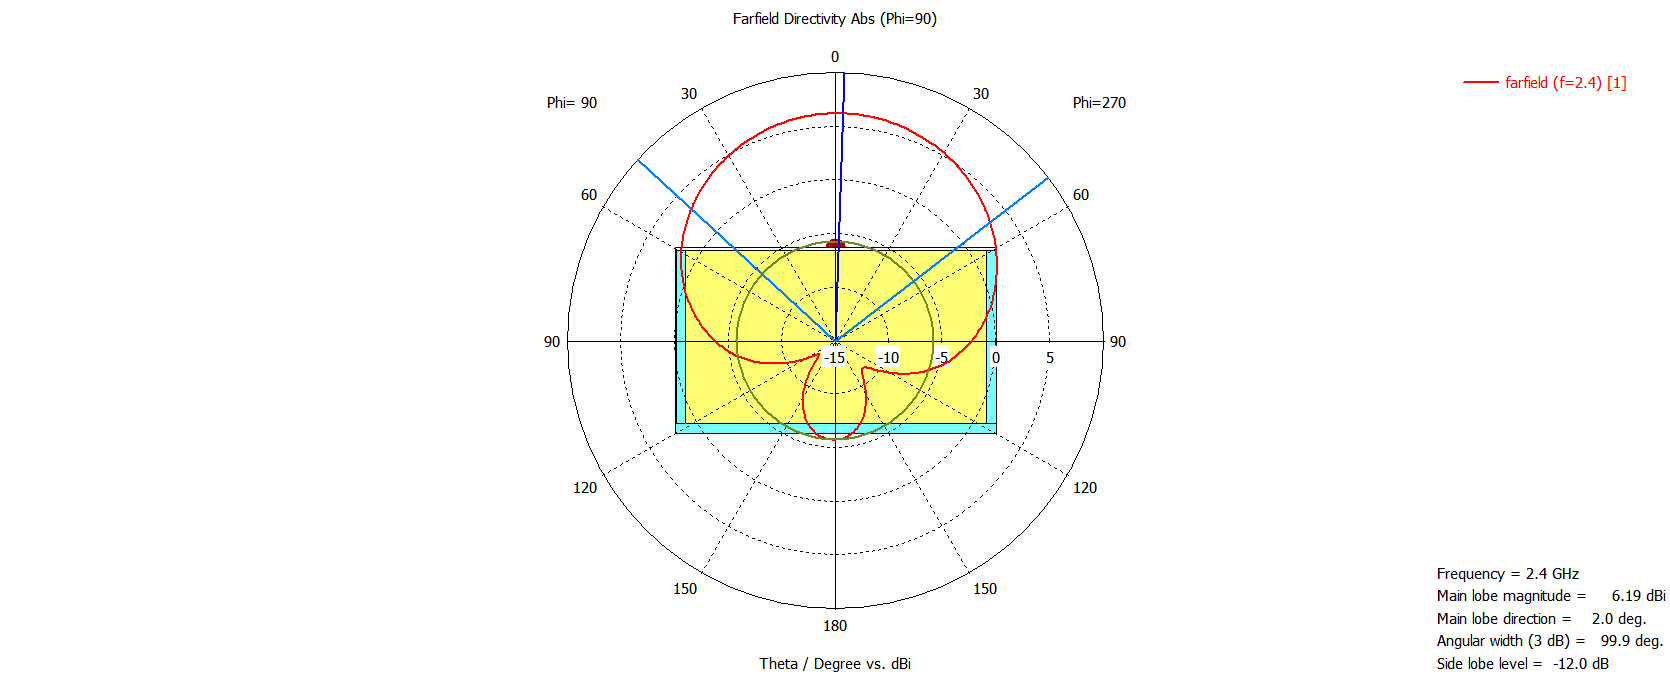
\includegraphics[width=0.9\linewidth]{figs/ch3_farfield1D.png}
    \caption{Farlfield directivity in 1D for Phi = 90}
    \label{fig:ch3_farfield1D.png}
\end{figure}

\par The gain of the antenna, as described by IEEE, is shown on Figure \ref{fig:ch3_gain.png}. We can see that its front facing gain, at $0^{\circ}$, is of $6.07\:\si{dB}$, and that it can attenuate the signal to the back, $180^{\circ}$, having a gain of $-5.90\:\si{dB}$.

\begin{figure}[H]
    \vspace*{0cm}
    \centering
    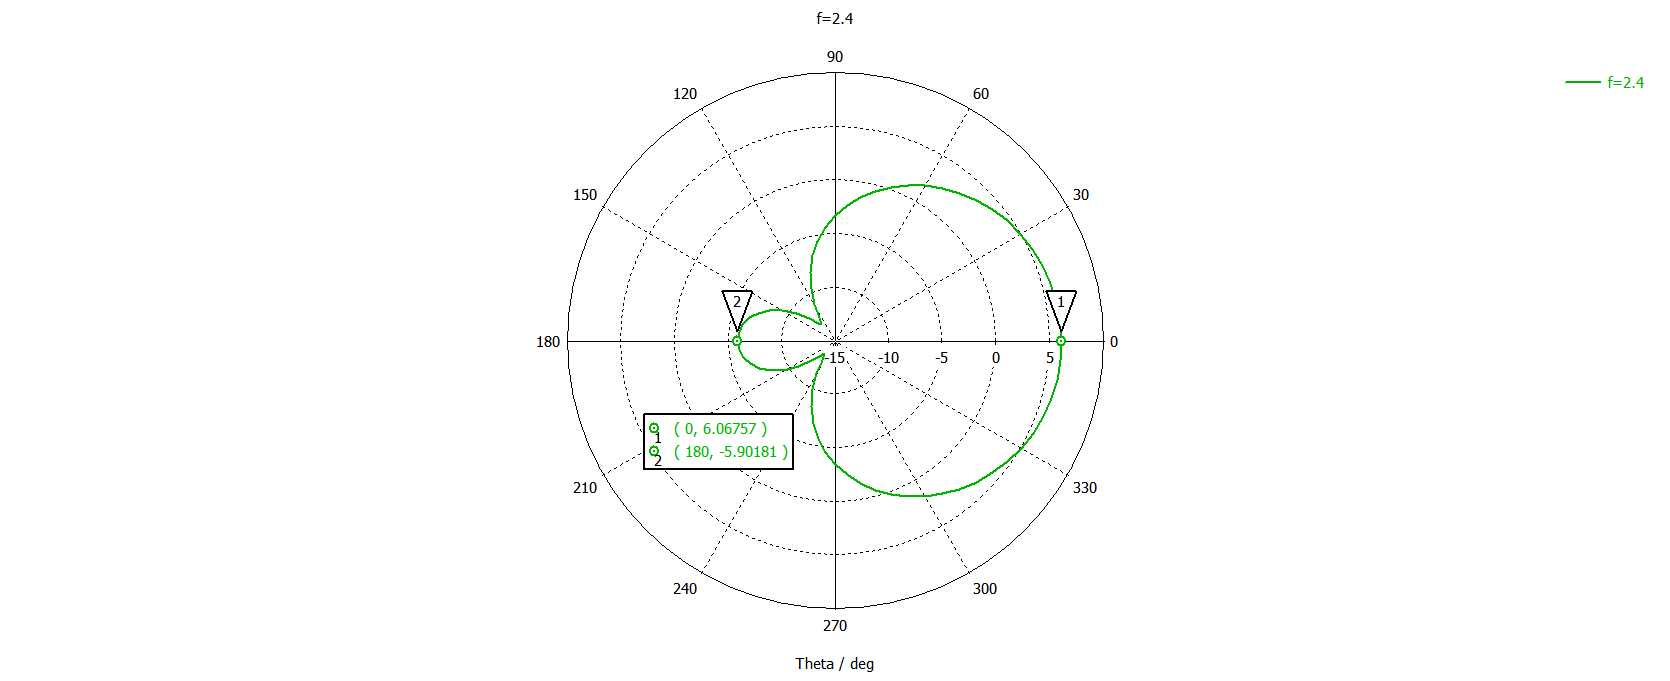
\includegraphics[width=0.9\linewidth]{figs/ch3_gain.png}
    \caption{Farlfield directivity in 1D for Phi = 90}
    \label{fig:ch3_gain.png}
\end{figure}

\par Afterwards, we decided to print two antennas. Instead of assembling both antennas at the same time, it was decided to do one at a time. The first was antenna 1 and the second was antenna 2. Both antennas were printed according to the same specifications. The box behind each antenna was also built according to the same dimensions. This eventually allowed us to improve antenna 2 based on the measurements of antenna 1.

\par The box from antenna 1 was made by soldering the sides of the box only on the corners, as can be seen on Figure \ref{fig:ch3_antenna1Box.jpg}. 

\begin{figure}[H]
    \vspace*{0cm}
    \centering
    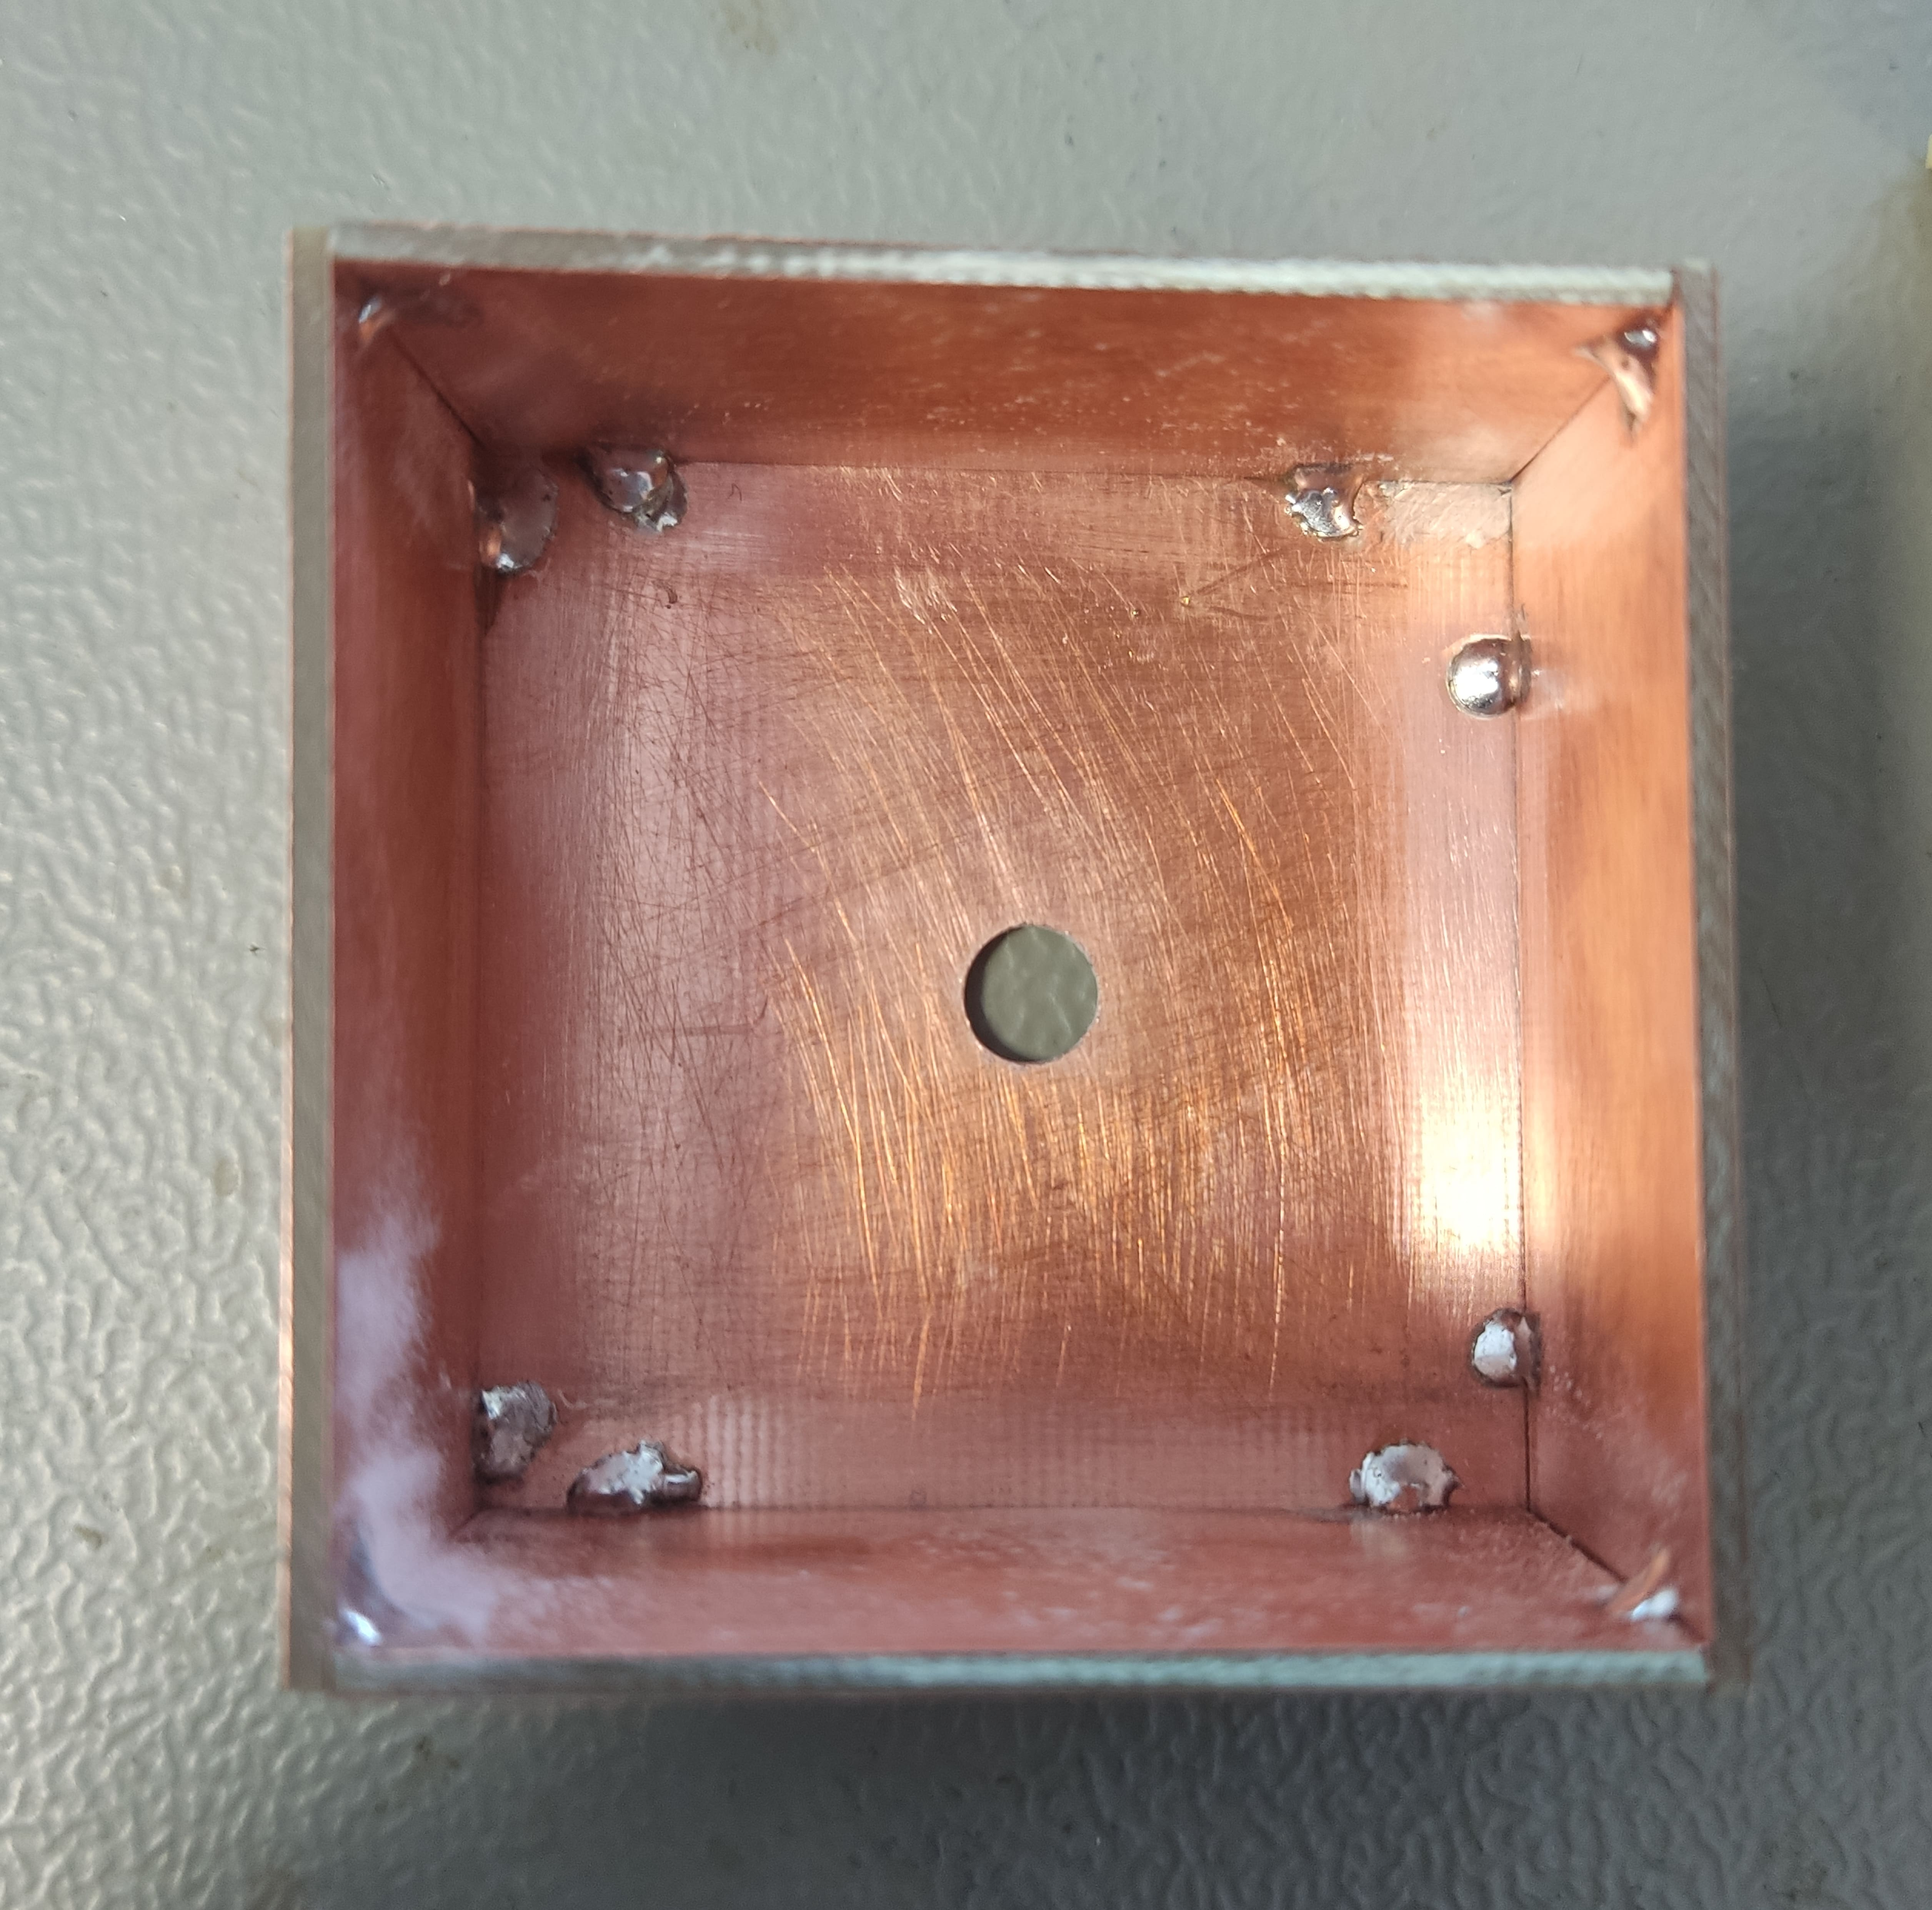
\includegraphics[width=0.3\linewidth]{figs/ch3_antenna1Box.jpg}
    \caption{Box part of antenna 1}
    \label{fig:ch3_antenna1Box.jpg}
\end{figure}

\par The antenna was fed by coaxial cable that would terminate in a front panel connector, as mentioned above. This can be seen in Figure \ref{fig:ch3_antennaFeedBack.png} and Figure \ref{fig:ch3_antennaFeedFront.png}.

\begin{figure}[H]
    \vspace*{0cm}
    \centering
    \includegraphics[width=0.3\linewidth]{figs/ch3_antennaFeedBack.png}
    \caption{Back side of antenna \ac{pcb} with feed cable}
    \label{fig:ch3_antennaFeedBack.png}
\end{figure}

\begin{figure}[H]
    \vspace*{0cm}
    \centering
    \includegraphics[width=0.3\linewidth]{figs/ch3_antennaFeedFront.png}
    \caption{Front side of antenna \ac{pcb} with feed point}
    \label{fig:ch3_antennaFeedFront.png}
\end{figure}

\par Both sides of antenna 1 were then glued together using commonly available super glue. Subsequently, the antenna was tested with a Keysight N9918A FieldFox Handheld Microwave Analyzer in the laboratories of Instituto de Telecomunicações, as seen in Figure \ref{fig:ch3_antenna1Testing.png}. The measured S11 results of this antenna can be seen in Figure \ref{fig:ch3_s11magAnt1.png}. We first started by calibrating the equipment and then captured the relevant values in the frequency range of $[1.5, 3.0] \:\si{GHz}$.

\begin{figure}[H]
    \vspace*{0cm}
    \centering
    \includegraphics[width=0.4\linewidth]{figs/ch3_antenna1Testing.png}
    \caption{S11 Magnitude results for antenna 1}
    \label{fig:ch3_antenna1Testing.png}
\end{figure}

\begin{figure}[H]
    \vspace*{0cm}
    \centering
    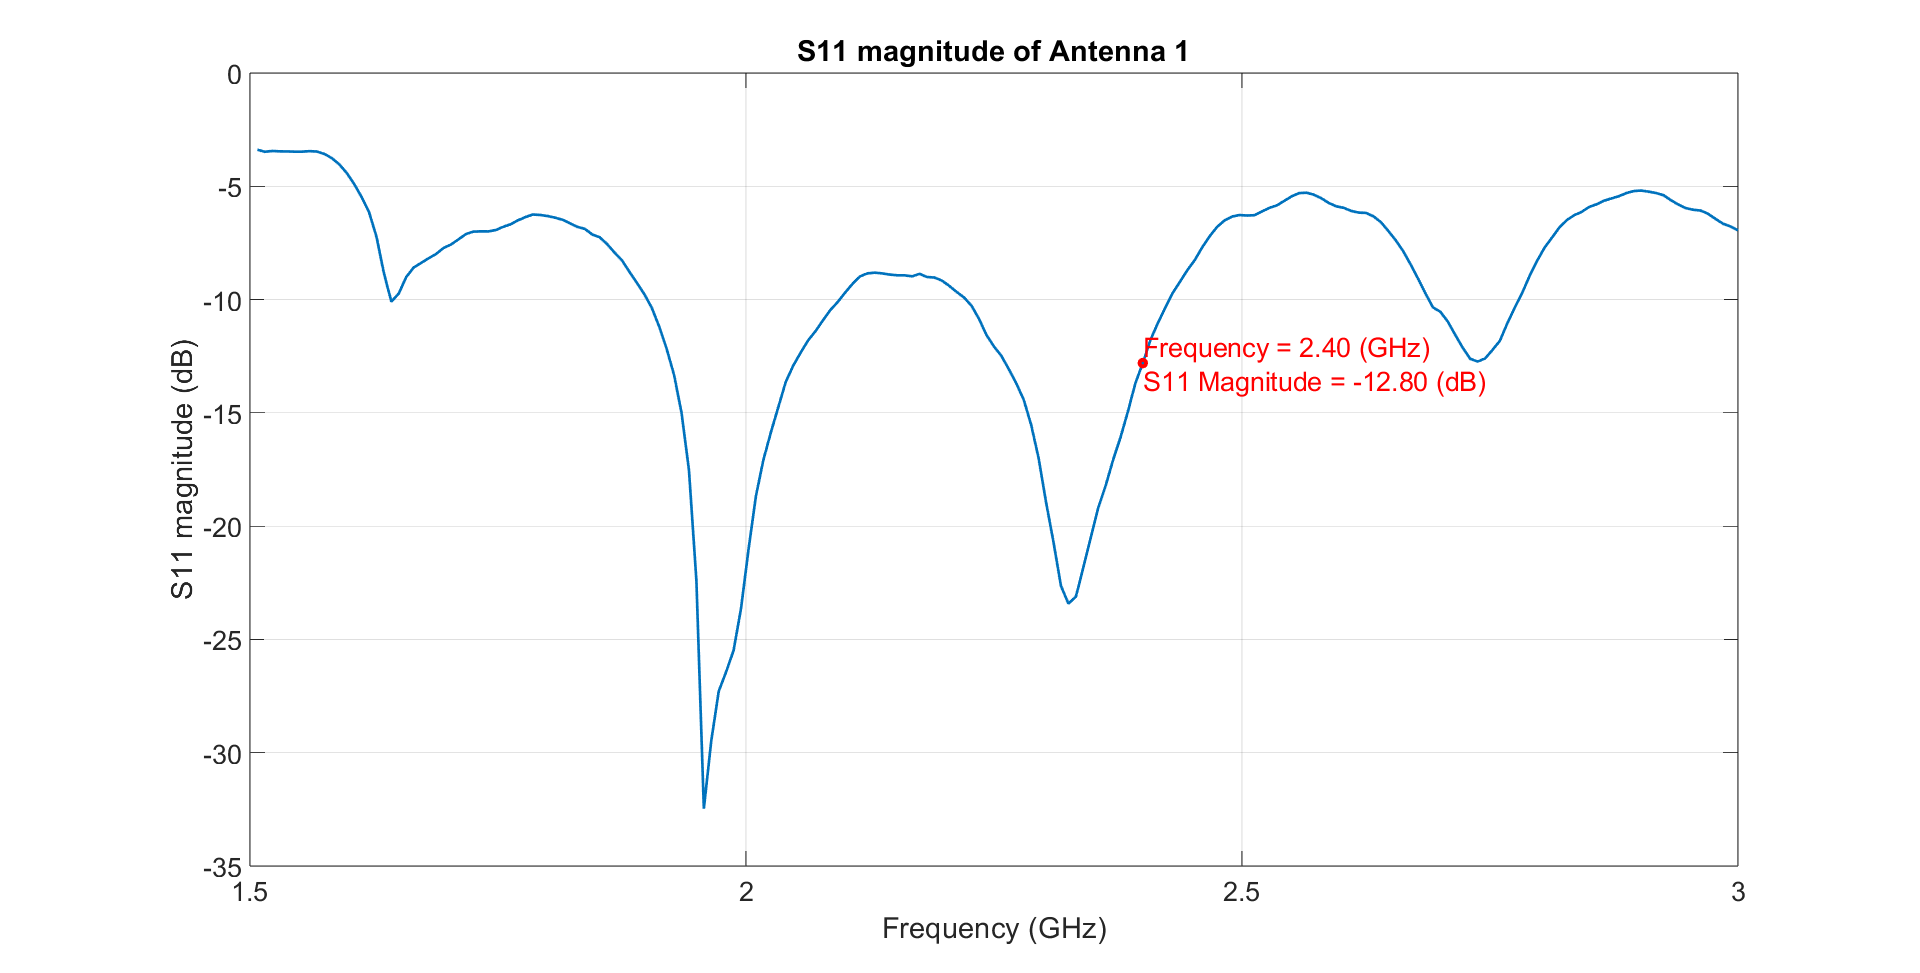
\includegraphics[width=1\linewidth]{figs/ch3_s11magAnt1.png}
    \caption{Testing of antenna 1}
    \label{fig:ch3_s11magAnt1.png}
\end{figure}

\par As can be seen, the results for this antenna were not what was expected from the simulations done on CST Studio. The S11 parameter is barely below the $-10 \:\si{dB}$ threshold, a value of $-12.80\:\si{dB}$ at a frequency of $2.4\:\si{GHz}$, and the overall response of antenna 1 was not good. After careful consideration, it was argued that maybe adding more soldering points inside the box could be beneficial, as it was suspected that the radiation from the backside of the antenna could be causing abnormal currents on the box's copper surface, and thus destroying the antenna's response. After this theory was proposed, the antenna 2 box was assembled and more solder points were added to the back portion of the box to achieve better results. The interior of the antenna 2 box can be seen in Figure \ref{fig:ch3_antenna2Box.jpg}.

\begin{figure}[H]
    \vspace*{0cm}
    \centering
    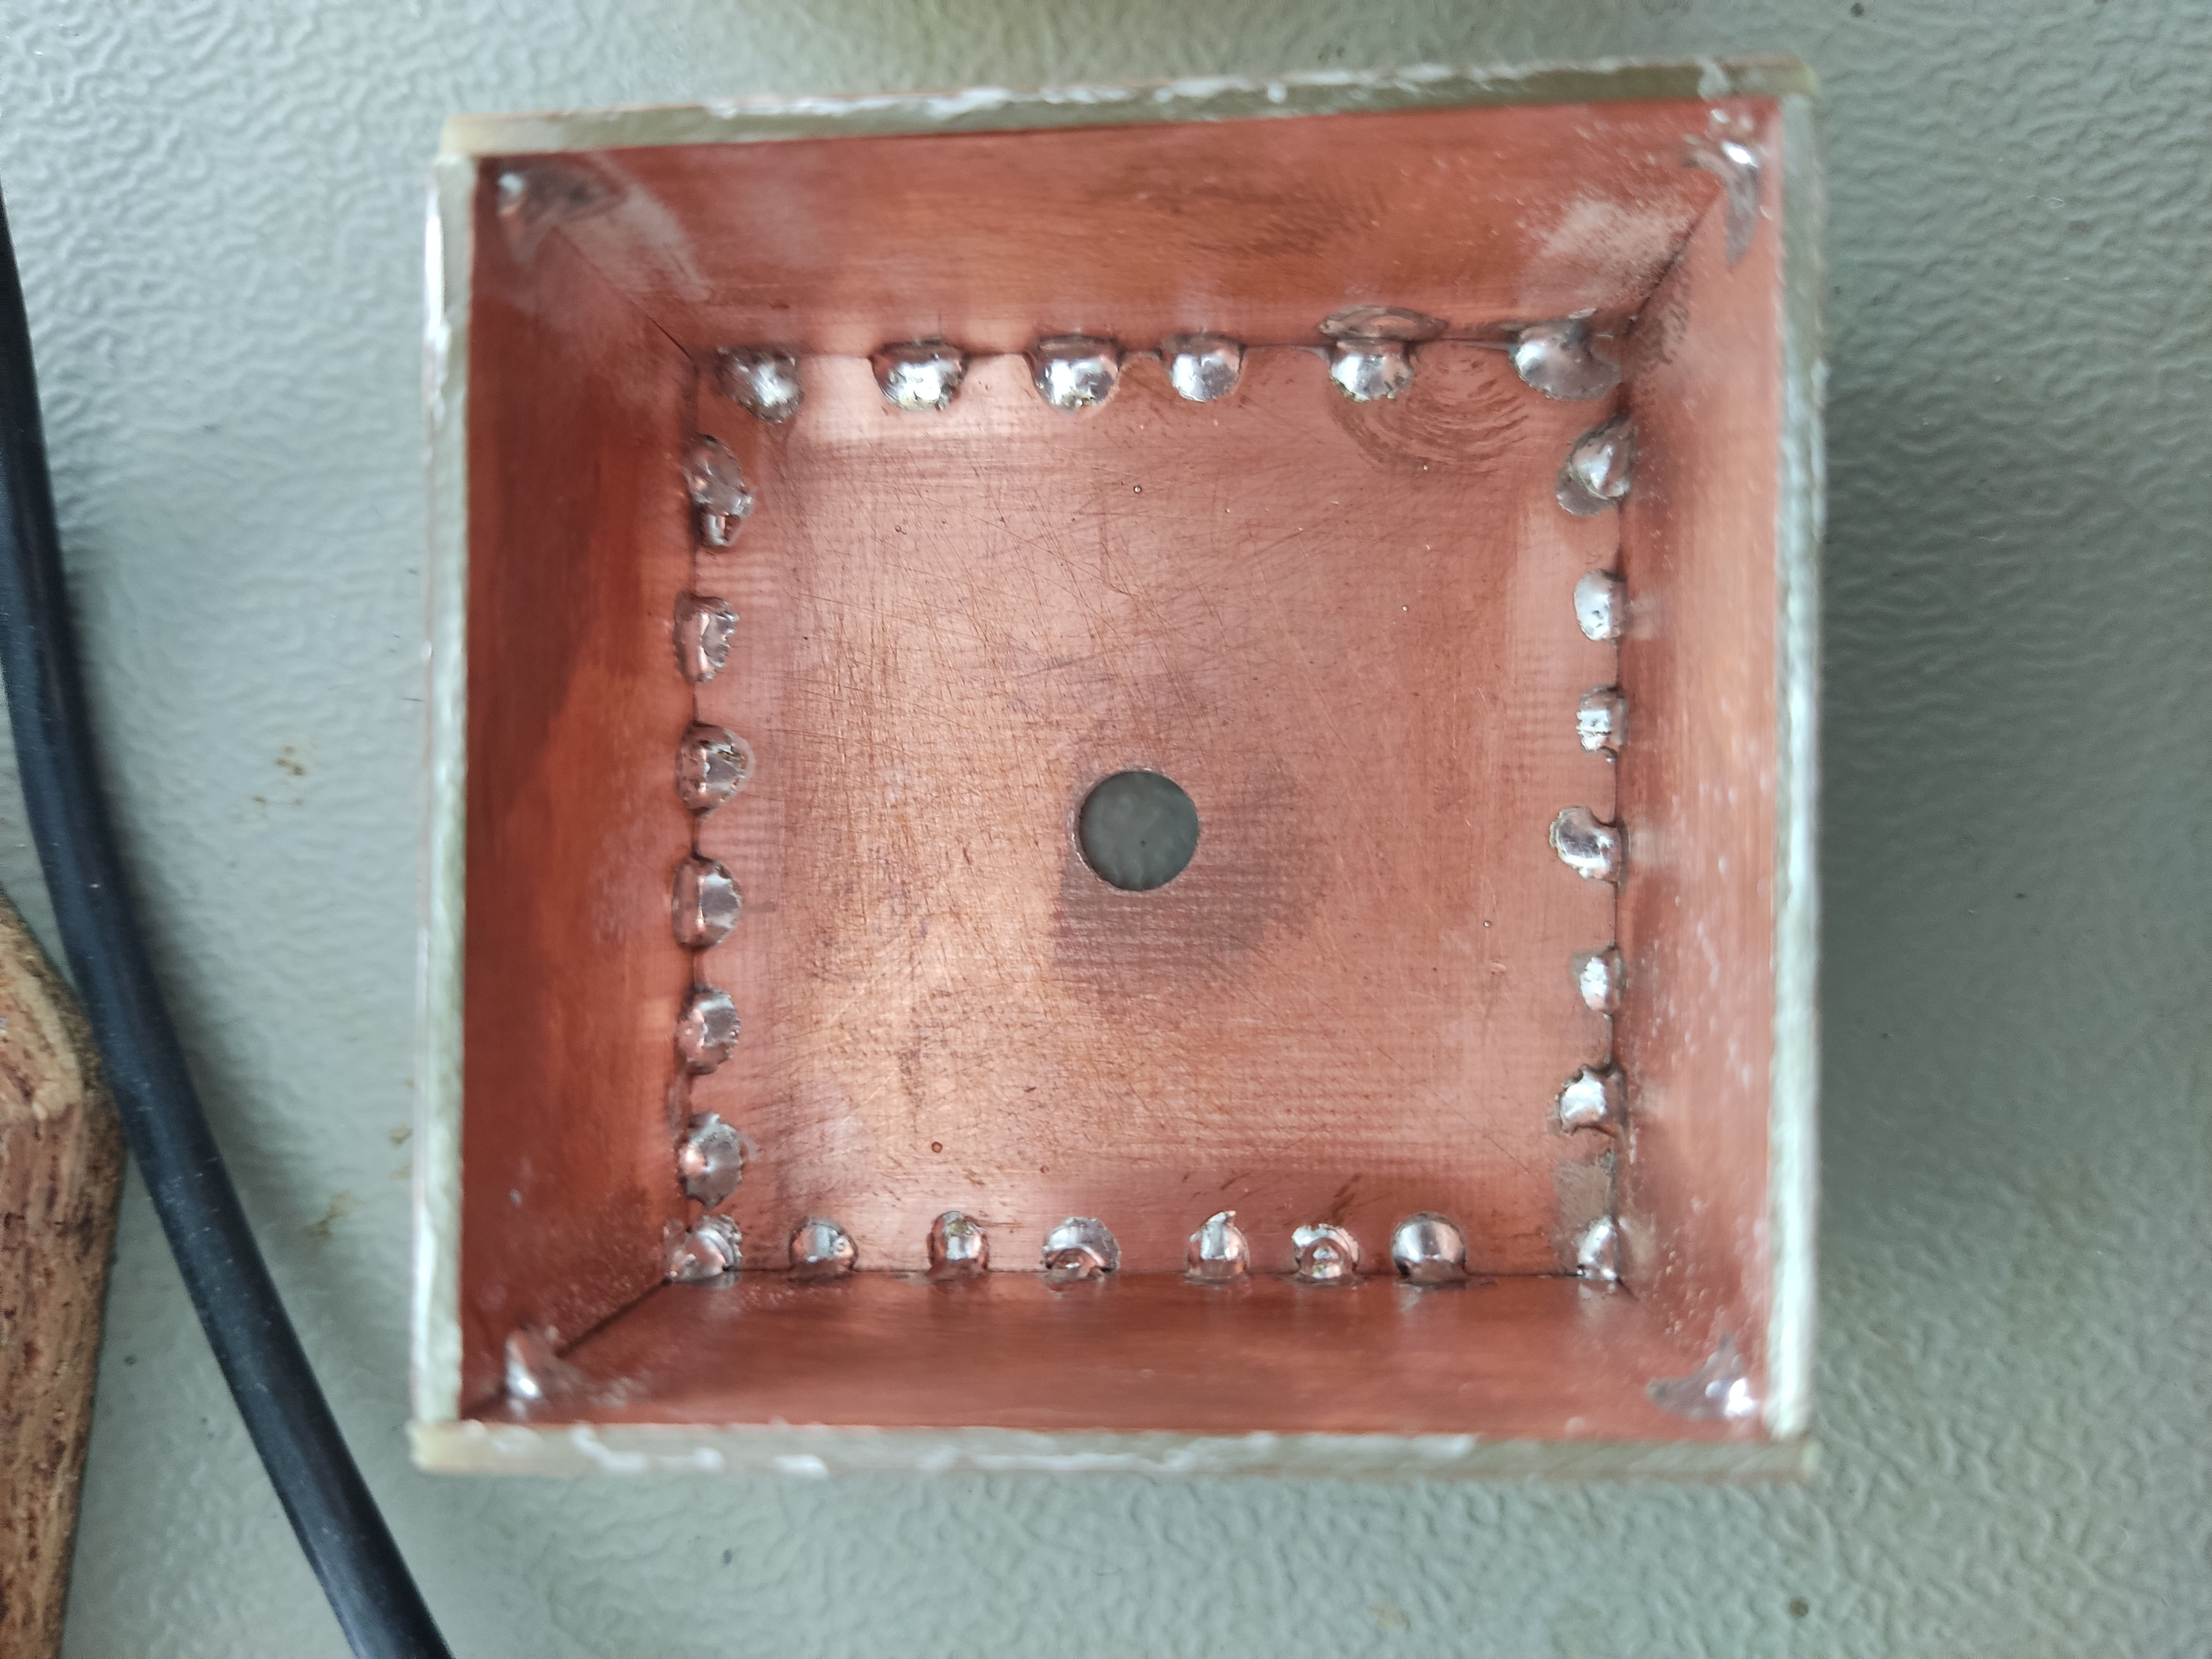
\includegraphics[width=0.3\linewidth]{figs/ch3_antenna2Box.jpg}
    \caption{View from the inside of antenna 2 box}
    \label{fig:ch3_antenna2Box.jpg}
\end{figure}

\par Antenna 2 has, in fact, better S11 Magnitude values, seen in Figure \ref{fig:ch3_s11magAnt2.png}, than antenna 1. This can be due to a variety of factors, as these antennas and the box behind them were hand made so there will differences in their construction. It cannot be determined that simply adding the extra solder points are the reason behind the improvements seen in antenna 2.

\begin{figure}[H]
    \vspace*{0cm}
    \centering
    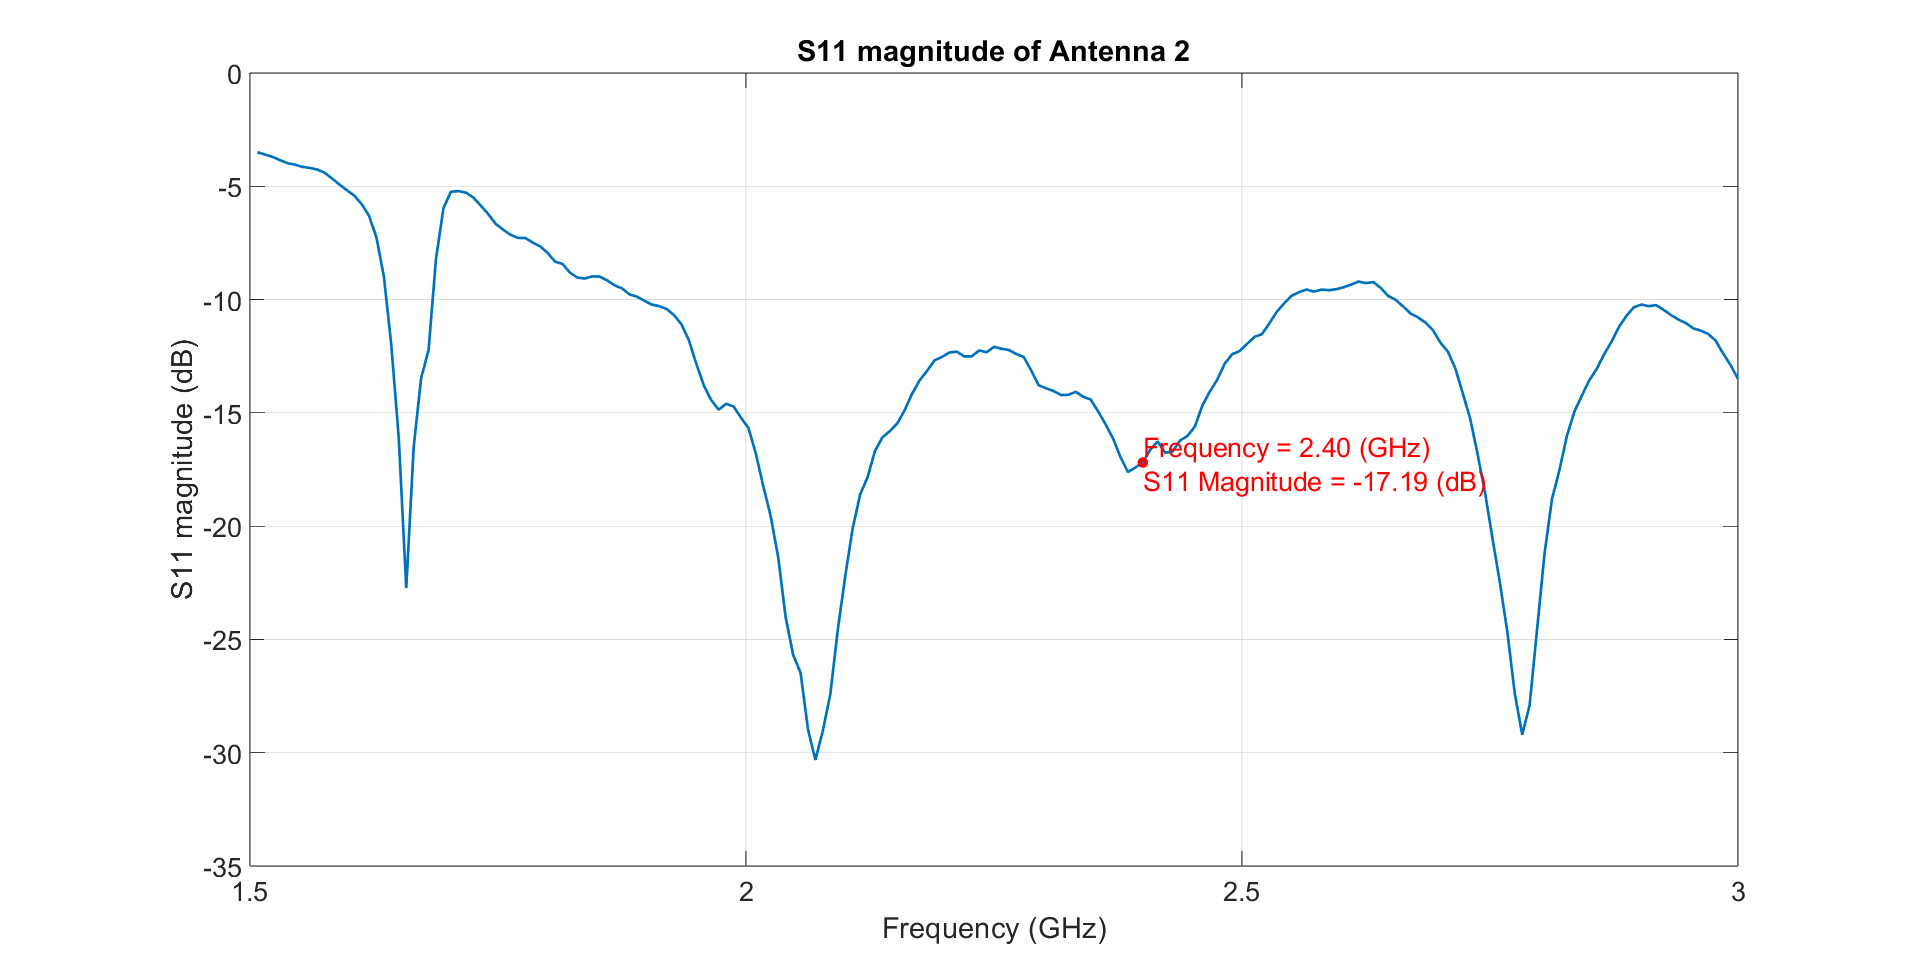
\includegraphics[width=1\linewidth]{figs/ch3_s11magAnt2.png}
    \caption{S11 Magnitude results for antenna 2}
    \label{fig:ch3_s11magAnt2.png}
\end{figure}

\par The response of antenna 2 has a larger portion of its S11 Magnitude below the $-10\:\si{dB}$ mark, managing to achieve a value of $-17.19\:\si{dB}$ at the $2.4\:\si{GHz}$ frequency. These results are also much closer to the simulated Magnitude of the S11 parameter done in CST Studio. This results in a more suitable antenna for application on the project.